\documentclass[12pt,a4paper,twoside,openany]{book}

%%% work %%%

% definice promenne docmode - print or screen mode
\newcommand{\visualmode}[1]{
	\def\docmode{#1}
	} 

% definice promenne langmode - czech or english mode
\newcommand{\thesislanguage}[1]{
	\def\thelanguage{#1} %czech/english
}

% autor prace
\newcommand{\thesisauthor}[1]{
	\def\theauthor{#1}
	\def\theciteauthor{\StrBehind{#1}{ }[\temp]\uppercase\expandafter{\temp}, \StrLeft{#1}{1}.}
}

% vedouci prace
\newcommand{\thesissupervisor}[1]{
	\def\thethesissupervisor{#1}
}

% nazev prace
\newcommand{\thesistitle}[1]{
	\def\thethesistitle{#1}
}


% vlozi titulni list a zadani
\newcommand{\VUTtitle}[2]{
	\pagestyle{empty}
	\includepdf[pages={1}]{#1}
	\ifthenelse{\equal{\docmode}{print}}{\newpage\phantom{blabla}}
	 
	\ifthenelse{\equal{#2}{blank}}
	{
	\newpage\phantom{blabla}
	\newpage\phantom{blabla}
	}{
	\includepdf[pages={1,2}]{#2}}
	} 

% abstrakt + klicova slova + citace
\newcommand{\abstract}[5]{
	\pagestyle{empty}
	\newpage
	\section*{Abstract}
	#1
	\section*{Summary}
	#2
	\vspace{20mm}\\
	\section*{Kl\'{i}\v{c}ov\'{a} slova}
	#3
	\section*{Keywords}
	#4
	\vfill
	\ifthenelse{\equal{\thelanguage}{czech}}{
	\section*{Bibliografick\'{a} Citace}
	\theciteauthor \textit{ \thethesistitle}. Brno: Vysok\'{e} u\v{c}en\'{i} technick\'{e} v Brn\v{e}, Fakulta strojn\'{i}ho in\v{z}en\'{y}rstv\'{i}, \the\year. \pageref{LastPage} s., Vedouc\'{i} diplomov\'{e} pr\'{a}ce: \thethesissupervisor.	
	}{
	\section*{Bibliographic citation}
	\theciteauthor \textit{ \thethesistitle}. Brno: Brno University of Technology, Faculty of Mechanical Engineering, \the\year. \pageref{MyLastPage} pages, Master's thesis supervisor: \thethesissupervisor.
	}
    \newpage
    \section*{Roz\v{s}\'{i}ren\'{y} abstrakt}
    #5
    \ifthenelse{\equal{\docmode}{print}}{\newpage\phantom{}} % blank page
	}
	
	
%	BRABLC, M. \textit{Control of Nonlinear Systems using Local Approximation Methods}. Brno, the Czech Republic: Brno University of Technology, Faculty of mechanical engineering, 2016. \pageref{LastPage} pages. Master's thesis, supervisor: doc. Ing. Robert Grepl, PhD..

% prohlaseni + podekovani
\newcommand{\acknowledgements}[2]{
	\pagestyle{empty}
	\newpage\phantom{blabla}
	\vfill
	#1
	\begin{flushright}
		\textbf{\theauthor}\\
		\vspace{1.5cm}
		\large{Brno} . . . . . . . . . . . . . \hfill . . . . . . . . . . . . . . . . .
	\end{flushright}

	\newpage\phantom{blabla}
	\ifthenelse{\equal{\docmode}{print}}{\newpage\phantom{blabla}}\phantom{}
	\vfill
	#2
	\begin{flushright}
		\textbf{\theauthor}
	\end{flushright}
	\ifthenelse{\equal{\docmode}{print}}{\newpage\phantom{blabla}\newpage}
	\newpage
	}

% nastaveni stylu stranky	
\newcommand{\vutpagestyle}{%[1]{
	
	\ifthenelse{\equal{\thelanguage}{czech}}{
		\selectlanguage{czech}
	}{
		\selectlanguage{english}
	}
	
	
	\setcounter{page}{7}
	\pagestyle{plain}
	\renewcommand{\baselinestretch}{1.5}
	\renewcommand{\chaptermark}[1]{\markboth{\MakeUppercase{\thechapter\ ##1}}{}}
	\renewcommand{\sectionmark}[1]{\markright{\MakeUppercase{\thesection\ ##1}}{}}
	\setlength{\abovedisplayskip}{0cm} % skip between equation and text
	\setlength{\belowdisplayskip}{0.5cm} % skip between equation and text
	\setlength{\abovedisplayshortskip}{0cm} % skip between equation and text
	\setlength{\belowdisplayshortskip}{0.5cm} % skip between equation and text
	\setlength{\textfloatsep}{0.5cm} % step between text and figure/table on top of the page
	\setlength{\intextsep}{0.5cm} % step between text and figure/table in text
	\tableofcontents
	\newpage
	\fancyhead{}
	\fancyfoot{}
	\ifthenelse{\equal{\docmode}{print}}
	{
	\fancyhead[LE,RO]{\leftmark}
	\fancyhead[LO,RE]{\rightmark}
	\fancyfoot[RO]{\thepage}
	\fancyfoot[LE]{\thepage}
	}{
	\fancyhead[L]{\leftmark}
	\fancyhead[R]{\rightmark}
	\fancyfoot[C]{\thepage}
	}
}

%\newcommand*{\fullref}[1]{\hyperref[{#1}]{Appendix \nameref*{#1}}} % named refference - no number
%\newcommand*{\fullref}[1]{\hyperref[{#1}]{\autoref*{#1} \nameref*{#1}}} % nambed reference - number

	


\usepackage{subcaption}
\usepackage{graphicx}
\graphicspath{{img/}{../img/}{../../img/}}
\usepackage{caption}
\usepackage{amsmath}

\usepackage{xargs}
\usepackage[pdftex,dvipsnames]{xcolor}  % Coloured text etc.
\usepackage[colorinlistoftodos,prependcaption,textsize=tiny]{todonotes}
%\usepackage{cite}

% Mode:
%\visualmode{print} % print mode 
\visualmode{screen} % screen mode 


% Language:
%\thesislanguage{czech}
\thesislanguage{english}

\thesisauthor{Artyom Voronin}
\thesissupervisor{Martin Brablc}
\thesistitle{Predictive maintenance of pneumatic pistons }


%% included paskages
\usepackage{pdfpages}
\usepackage{xifthen}
\usepackage{fancyhdr}
\usepackage{lastpage} 
\usepackage{titlesec} % allows title formating
\usepackage{lipsum} % some latin text for examples
\usepackage[nottoc]{tocbibind} % add othe chapters (bibliography) to ToC
\usepackage[framed]{mcode} % add formated matlab code
\usepackage{mathtools} % math signs and tools
\usepackage{multicol} % merge columns in table
\usepackage{multirow} % merge rows in table
\usepackage{bm} % bold signs in equations
\usepackage[font=small,skip=0pt]{caption} % smaller distance between caption and figure/table
\usepackage{xstring} % string processing

%% Optional
\usepackage{amssymb} % math signs (check sign)
\usepackage{epstopdf} % allows esp include
\usepackage[shortlabels]{enumitem} % allows itemize indent options
\usepackage{bbding} % special signs (\Checkmark, \XSolidBrush)
%\def\labelitemi{--} % change itmize default marker

\usepackage{setspace}
\usepackage[hang,flushmargin]{footmisc} % footnotes without indentation

%% style settings

% symetrical / asymetrical margins
% a4 size is 210 mm x 297 mm, print size is 170 mm x 250 mm
% \ifthenelse{\equal{\docmode}{print}} 
% {\usepackage[top=2.4cm, bottom=2.3cm, left=1.5cm, right=1.5cm, bindingoffset=10mm]{geometry}}
% {\usepackage[top=2.4cm, bottom=2.3cm, left=2cm, right=2cm, bindingoffset=0mm]{geometry}}

%original VUT print size - 160 mm x 240 mm
\ifthenelse{\equal{\docmode}{print}} 
{\usepackage[top=2.9cm, bottom=2.8cm, left=2cm, right=2cm, bindingoffset=10mm]{geometry}}
{\usepackage[top=2.9cm, bottom=2.8cm, left=2.5cm, right=2.5cm, bindingoffset=0mm]{geometry}}


% title formats
\titleformat{\chapter}[hang]{\Huge\bfseries}{\thechapter}{5mm}{\Huge\bfseries}
\titleformat{\section}[hang]{\Large\bfseries\setstretch{0.6}}{\thesection}{5mm}{\Large\bfseries}
\titleformat{\subsection}[hang]{\large\bfseries\setstretch{0.6}}{\thesubsection}{5mm}{\normalsize\bfseries}

\titlespacing*{\chapter}{0cm}{0cm}{1.5cm} % {command}{left}{before}{after}
\titlespacing*{\section}{0cm}{0.5cm}{0.3cm}
\titlespacing*{\subsection}{0cm}{0.3cm}{0.3cm}

\setlength{\parskip}{0pt} % changes vertical space between paragraphs
\setlength{\headheight}{16pt}

% coloring format
\usepackage[pdftitle={Masters Thesis},
pdfauthor={\theauthor},
%pdftex=true,
%bookmarks=true,a4paper]
linkcolor=black,
colorlinks=true,
breaklinks=true,
urlcolor=black,
citecolor=black,
unicode]%,a4paper]
{hyperref}
%\usepackage[pdftex]{graphicx}
%\DeclareGraphicsExtensions{.png,.pdf,.eps,.bmp,.jpg,.emf}

%% language settings
\ifthenelse{\equal{\thelanguage}{czech}}{
	\usepackage[czech]{babel}
	\usepackage[utf8]{inputenc}
	\usepackage[T1]{fontenc}
	\usepackage{lmodern}


}{
	\usepackage[english,czech]{babel}
}


%% chapter foot/head style
%\ifthenelse{\equal{\docmode}{print}}
%{
%	\fancypagestyle{plain}{%
%		\fancyhead{}
%		\fancyfoot{}
%		\renewcommand{\headrulewidth}{0pt}% Line at the header invisible
%		\renewcommand{\footrulewidth}{0pt}% Line at the footer invisible
%		\fancyfoot[RO]{\thepage}
%		\fancyfoot[LE]{\thepage}
%	}
%}{
%	\fancypagestyle{plain}{%
%		\fancyhead{}
%		\fancyfoot{}
%		\renewcommand{\headrulewidth}{0pt}% Line at the header invisible
%		\renewcommand{\footrulewidth}{0pt}% Line at the footer invisible
%		\fancyfoot[C]{\thepage}
%	}
%}

 % nastaveni stylu dokumentu

\begin{document}
	
\VUTtitle{pages/titulni_color.pdf}{pages/zadani_color.pdf} 
%\VUTtitle{pages/titulni_color.pdf}{blank} % Use when print


\abstract{ % abstrakt cesky

Tato práce se zabývá vytvořením simulačního modelu dvojčinného
pneumatického pístu s mechanickou sestavou, včetně modelů snímačů, s
následujícím odhadem parametrů a aproximací chování demonstračního
zařízení. Dalším cílem je prezentace různých přístupů prediktivní údržby
na datové sadě měřené na demonstračním zařízení. Na
měřený datový soubor se aplikovaly signal-based techniky bez použití simulačního
modelu a model-based metody, které vyžadují použití simulačního
modelu.

Výsledkem této práce je ověření možnosti monitorování stavu zařízení pomocí
nainstalovaných senzorů a vyhodnocení efektivity senzorů z hlediska
přesnosti a finančních nákladů.

	}{ % abstrakt anglicky

This thesis deals with creating a simulation model of a double-acting
pneumatic piston with a mechanical assembly, including the sensors models,
with the following parameter estimation and approximation to the behavior
of a demonstration device. Another goal is the demonstration of various
Predictive Maintenance approaches on a dataset measured on a demonstration
device. Applying signal-based techniques to the measured dataset without using
a simulation model and a model-based method that requires the use of a
simulation model. 

The outcome of this work is the verification of the possibility of
monitoring the device's condition state,  using installed sensors, and
evaluating the efficiency of the sensors in terms of accuracy/cost. 
	}{ % klicova slova česky
dvojčinný pneumatický válec, prediktivní údržba, identifikace a detekce
poruch, zbývající doba použitelnosti, PdM, FDI, RUL
	}{ % klicova slova anglicky
    double-acting pneumatic piston, predictive maintenance, fault detection
    and identification, remaining useful life, PdM, FDI, RUL 
    }{ 
    \subsection*{Uvod}

Od začátku průmyslové revoluce, složitost
výrobní stroje a sériové linky se postupně zvyšovaly a vyžadují
neustálé sledování podmínek systémů z ekonomických důvodů.
Na druhou stranu kritické systémy jako letadla, kosmické lodě,
automobilové systémy, jaderné reaktory a další vyžadují okamžitý poplach
chyba, lokalizovat došlo k chybě a ještě více předvídat možnou budoucnost
poruchy. Tyto požadavky se staly předpoklady pro detekci chyb
a pole Analýza a Prediktivní údržba.

Výrobní proces vždy zahrnoval prvky kontroly chyb a online
monitorování. Od prvních metod detekce poruch, například vizuální
inspekce, dnešní továrny přecházejí na automatizované systémy skládající se z
senzory a výpočetní jednotky k vyhodnocení poruch. Někdy je
kritické pro sledování zpracovatelského zařízení v reálném čase, aby nedošlo k poškození
způsobené chybou nebo anomálií. Každá jednotlivá chyba může způsobit zpomalení
výrobní proces a tím i snížení zisku.

Algoritmy monitorování zařízení v reálném čase vytvořily Fault Detection a
Pole analýzy (FDA). Metody FDA ve většině případů nevyžadují stroj
techniky učení a dokáže detekovat poruchy pomocí základních algoritmů
od Fourierovy analýzy a algoritmů pro kontrolu trendů po složitější
techniky, jako jsou Gaussovské modely směsí.

Vzhledem k množství údajů shromážděných v posledních letech a rozšíření
technologie ukládání dat jako cloudové služby a efektivita výpočtu, to
je možné používat pokročilejší algoritmy pro detekci poruch a
analýza. Pomocí technik klasifikace strojového učení je to možné
izolovat, kde se chyba vyskytuje. Další možnost, která se stane
k dispozici s velkým množstvím dat je odhad zbývajícího užitečného
život (RUL) celého systému. Tyto techniky vedly k predikci
údržba jako snaha o optimální řešení údržby. Aktuální
technický stav zařízení je vždy k dispozici podle informací
extrahované z měřených signálů. Je možné použít aktuální systém
podmínky pro odhad zbývající životnosti v čase nebo vzdálenosti
měření, jako jsou dny, kilometry nebo cykly. Odhadovaný zbytek
životnost dává možnost plánovat údržbu týkající se skutečného systému
podmínky.

Tyto zbývající algoritmy pro odhad životnosti, detekce poruch
metody a techniky modelování a identifikace systémů tvoří nový
pole prediktivní údržby.

Modelování systému umožňuje poskytovat experimenty a vyvíjet řešení
offline před fyzickými implementacemi hardwaru. Nedostupné nebo
náročné implementovat měření lze nahradit generovanými daty
ze simulačního modelu a nakonec pomáhá nasadit robustní algoritmus.

Tato práce poskytuje krátký úvod do detekce poruch a predikce
metodiky údržby a základní terminologie.
Kapitola \ref{ch: teor_surv} popisuje hlavní cíl a problémy
v těchto oblastech a zaměřuje se na podobnosti a rozdíly mezi nimi
dva přístupy.

Vývoj simulačního modelu dvojčinného pneumatického aktuátoru a
porovnání s reálným vybavením pomocí různých přístupů je
popsané v kapitolách 3, 4 a 5.

Následující kapitola 6 ilustruje prediktivní údržbu založenou na signálu
metody využívající různé senzory dostupné v demonstračním zařízení.
Aplikování předzpracování, extrakce funkcí a klasifikační model,
senzory byly hodnoceny z hlediska funkčnosti, přesnosti a ceny.

Techniky prediktivní údržby založené na modelu a simulační model
využití je demonstrováno v kapitole 7. Simulační model je zvyklý
určit zbytkové signály mezi naměřenými daty a simulací
výstup modelu. Pomocí simulačního modelu jsou také údaje o degradaci
generovány a použity při odhadu zbývající životnosti.

\subsection*{Závěr}
Cílem této práce bylo demonstrovat a ověřit detekci poruch a
techniky prediktivní údržby na dvojčinném pneumatickém pístu
montáž jako objekt případové studie.

\subsubsection*{Simulační model}

Jedním z výstupů práce je simulační model
dvojčinný pneumatický pístový systém postavený na základě diferenciálních rovnic
z pneumaticko-mechanické oblasti, modelováno a vyvíjeno pomocí
Software Matlab/Simulink. Simulační model byl odhadnut pomocí
parametry zdravého chování systému. Existuje však možnost
přehodnotit parametry do poruchového stavu a simulovat systém při poruše
stav.

Vzhledem k dostupným naměřeným údajům a výrazně nelineární dynamice
systému, simulační model vykazuje dobrou shodu s naměřeným
data. Na rozdíl od modelu vytvořeného pomocí knihovny Simulink / Simscape je
výrazně méně výpočetně nákladné při zachování číselné hodnoty
stabilita. Tato fakta jsou zásadní, když je odhad parametrů v
pokrok.

Simulační model byl použit k experimentování s chováním systému v systému
různé podmínky, modelovat poruchové situace a generovat data pro návrh
a vyvíjet robustní algoritmy prediktivní údržby.


\subsubsection{Signal-based PdM}
Dalším výstupem je ověření možnosti klasifikace a
detekce poruchového stavu pomocí technik prediktivní údržby,
pomocí metod založených na signálu a modelu.
 
Pokusy byly prováděny na datové sadě měřené na demonstraci
zařízení pomocí sedmi typů senzorů.
  
Metoda založená na signálu je založena na extrakci užitečných informací
přímo ze signálu v časově-frekvenčních doménách. Každý senzor vyžadoval
individuální přístup k předzpracování, extrahování funkcí, hodnocení
vlastnosti a vytváření klasifikačních modelů. Ale obecně existuje
minimální předběžné zpracování potřebné k uchování možných užitečných informací.

Tabulka \ref{sensors_final} obsahuje srovnání čidel ve 2
kategorie, přesnost provedená v datovém souboru testu a náklady na senzory. The
graph \ref{fig:sensors_final_bar} vizualizuje tato data.

Překvapivě všechny senzory vykazovaly přesnost více než 75 \%. Mikrofony
nabízejí vynikající výkon z hlediska nákladů a přesnosti a jsou
vhodné pro instalaci a údržbu.

\begin{figure}[h!]
    \centering
    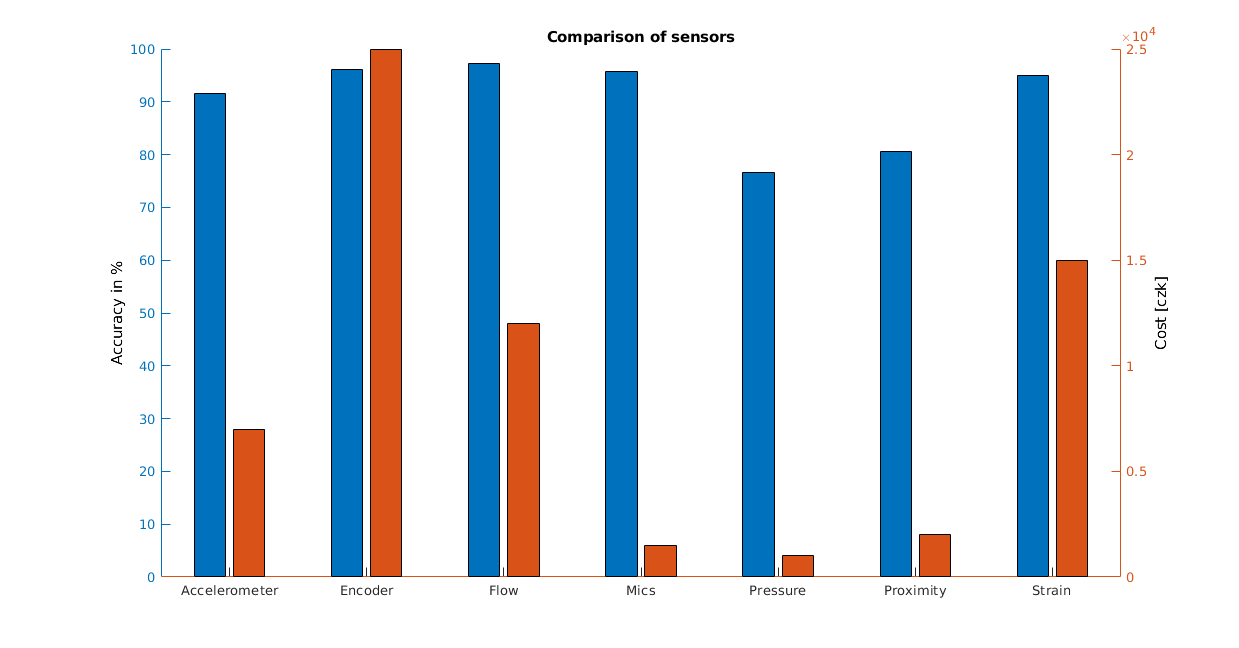
\includegraphics[width=1\textwidth]{sensors_final_bar.png}
    \caption{Comparison of sensors from accuracy/cost perspective}
    \label{fig:sensors_final_bar}
\end{figure}

\begin{table}[h]
    \centering
    \begin{tabular}{|c|c|c|c|c|c|c|c|}
        \hline
        \textbf{Sensor}   & Acc & Encoder & Flow & Mics & Pressure & Proximity & Strain \\
        \hline
        \textbf{Accuracy [\%]} & 91.6 & 96.1 & 97.2 & 95.8 & 76.6 & 80.5 & 95.0 \\
        \hline
        \textbf{Cost [czk]} & 2x 3500 & 25000 & 6000 & 3x 500 & 1000 & 2x 1000 & 15000 \\
        \hline
    \end{tabular}
    \caption{Comparison of sensors from accuracy/cost perspective}
    \label{tab:sensors_final}
\end{table}

\subsubsection*{PdM podle modelu}

Další částí této práce bylo aplikovat modelové metody a použití a
simulační model pro algoritmy prediktivní údržby. Tyto algoritmy
jsou praktické, když je těžké extrahovat užitečné informace pomocí a
metoda založená na signálu. Nebo je to vhodné v některých případech, pokud tomu rozumíme
dynamiku systému a umím využívat některé systémové proměnné jako
indikátory stavu.

Použití metody extrakce funkcí ve formě nelineární
koeficient identifikačního modelu systému, konkrétně s
Hammerstein-Wiener model, nedal spolehlivé výsledky. Extrahované funkce
nemají statistickou závislost a je nemožné předvídat typ poruchy
použitím této metody na naměřených datech z pneumatického pístu jako případ
studie.

Na druhou stranu zbytkový odhad pomocí simulačního modelu
ukázal vynikající výsledky. Měřený signál polohy byl porovnán s
signál ze simulačního modelu v normálním chování. Tento zbytek
signál byl použit ke klasifikaci poruchového stavu a dosažení 99 \% na a
menší datová sada. Ale vzhledem k výsledkům získaným pomocí signálu
Metoda zbytkového odhadu se může zdát zbytečná. V tomhle
konkrétního případu, z praktického hlediska, zlepšení
výsledek o několik procent nepřináší zásadní změny, ale
doba výpočtu se významně zvyšuje.

Byla také ověřena možnost poruch modelování a simulace senzorů
pomocí simulačního modelu. I když je náročné sbírat chyby
data ze snímače v reálných podmínkách mohou být generována data o poruše
od simulačního modelu a dokonce v kombinaci s primární datovou sadou do
vytvořit syntetický datový soubor.

\subsubsection*{RUL}

Jedním z hlavních cílů prediktivní údržby je odhadnout
zbývající životnost. Původní datová sada neobsahuje záznam o
historická data, která ukazují degradační chování.

Běžným problémem při údržbě pneumatických ovladačů je netěsnost
vzduchu z komory, kde je umístěn píst. Tato situace byla
modelované na simulačním modelu a generovaná data byla použita pro RUL
odhad.

Vygenerovaná datová sada obsahuje 25 simulací s různými poruchami
dynamika. Každá simulace zahrnuje jiný počet cyklů v závislosti na tom
na dynamiku selhání, než dojde k selhání systému. Každý cyklus
obsahuje 10sekundové měření odezvy systému. V
experimentu byl jako předmět zájmu vybrán signál toku. Z
signálu toku, byl vypočítán parametr tvarového faktoru a použit jako a
indikátor stavu.

Výsledkem je, že je možné odhadnout zbývající životnost
generovaný datový soubor degradace pomocí modelu zbytkové podobnosti,
model párové podobnosti a model lineární degradace. Předpověď
výsledky jsou uspokojivé.

\subsubsection*{Další vývoj}

Jako další vývoj by bylo vhodné modelovat odhad
parametry systému po částech ke zlepšení výsledků, s důrazem na
vlastnosti škrticích ventilů a tlumičů s úpravami.

Proveďte měření stavu poruchy úniku vzduchu a sbírejte historické údaje
údaje o degradaci skutečného pneumatického pístu. Následně vyhodnotit
dynamika poruchy způsobené únikem vzduchu. Ověřte možnost
odhad zbývající životnosti pomocí snímače průtoku. Může to být
zajímavá případová studie k ověření možnosti použití odhadu RUL
mikrofony. Pokud je výkon dostupných senzorů nedostatečný,
lze provádět měření tlaku v komoře. Tlak v
komora je přímo závislá na úniku vzduchu z komory, jako
uvedené v rovnici \ref{}. Příklad změn tlaku z
simulační model je znázorněn na obrázku \ref{}.

	} % vyrobi i citaci

\acknowledgements{
    I hereby declare that except where specific reference is made to the work of others,
    the contents of this dissertation are original and have not been submitted in whole or in
    part for consideration for any other degree or qualification in this, or any other university.
    This master’s thesis is my own work and contains nothing which is the outcome of work
    done in collaboration with others.
	}{
	Poděkování..
	} % vlozi prohlaseni a podekovani


\vutpagestyle % prepise styl stranky, vlozi obsah


\chapter{Introduction}

 
%% Artyom Voronin
%%  __     _ _                   
%% / _| __| (_)  _ __  _ __ ___  
%%| |_ / _` | | | '_ \| '_ ` _ \ 
%%|  _| (_| | | | |_) | | | | | |
%%|_|  \__,_|_| | .__/|_| |_| |_|
%%              |_|              
%% Brno, 2021

\documentclass[class=article, crop=false]{standalone}
\usepackage[subpreambles=true]{standalone}
\usepackage{subcaption}

\usepackage{sectsty}
\usepackage{graphicx}
\graphicspath{{img/}{../img/}{../../img/}}
\usepackage{listings}
\lstset{language=Matlab}
\usepackage{hyperref}
\usepackage{amsmath}
\usepackage{import}
\usepackage{subfiles}
\usepackage[utf8]{inputenc}
\usepackage[english]{babel}

%\usepackage{todonotes}

%\usepackage[square, numbers]{natbib}
%\bibliographystyle{unsrtnat}
%\usepackage[nottoc]{tocbibind}

%\usepackage{biblatex}
%\addbibresource{./citations.bib} %usage \cite{test}
% Margins
% 
\topmargin=-0.45in
\evensidemargin=0in
\oddsidemargin=0in
\textwidth=6.5in
\textheight=9.0in
\headsep=0.25in

%\title{PM and FDI comparison}
%\author{Artyom Voronin} 
%\date{}

\begin{document}
\tableofcontents

% -----------------------------------------------------------------------------
% 
% -----------------------------------------------------------------------------
\section{Theoretical Survey}
The relative arrangement PM and FDI methods representing in following
figure \ref{fig:fdi_pm}
\begin{figure}[h!]
    \centering
    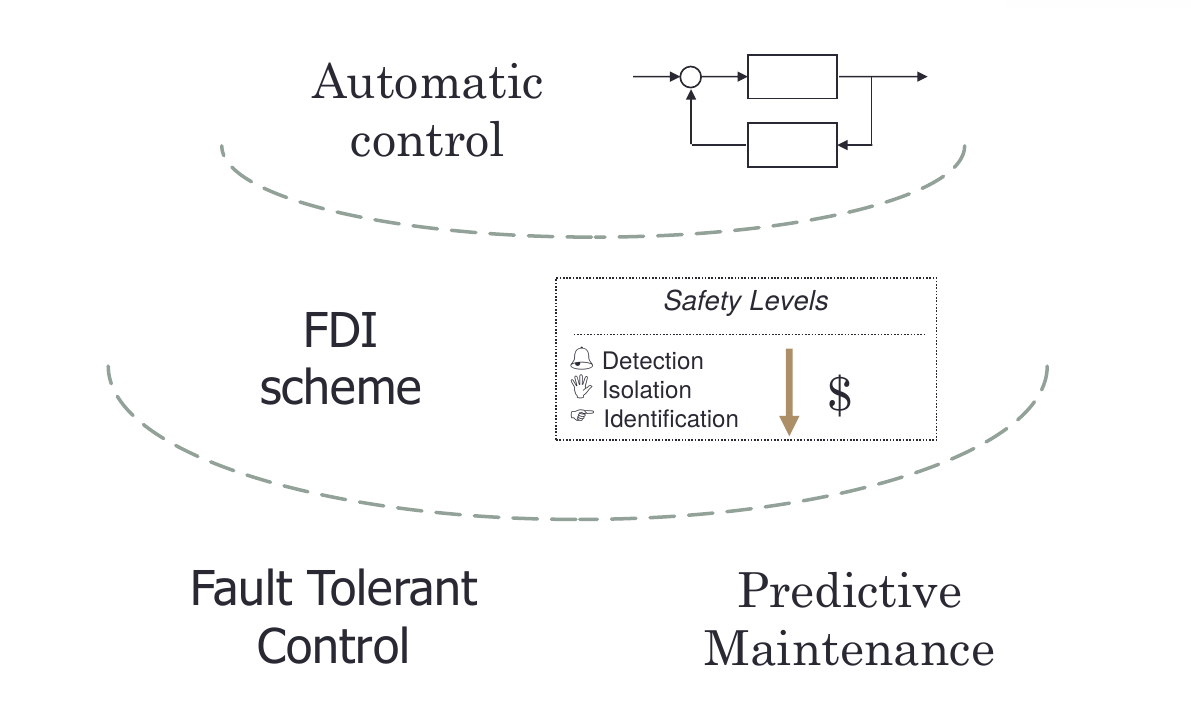
\includegraphics[scale=0.3]{FDI_PM.png}
    \caption{PM and FDI }
    \label{fig:fdi_pm}
\end{figure}

% -----------------------------------------------------------------------------
% 
% -----------------------------------------------------------------------------

\subsection{Problem Definition}
% XXX FaultDetectionMethods-ALiteratureSurvay.pdf
\begin{itemize}
    \item Fault
    \item Failure   
    \item Malfunction
\end{itemize}

\subsubsection{Types of Faults}
\begin{itemize}
    \item Plant
    \item Sensor
    \item Combination
\end{itemize}

\subsubsection{Types of Maintenance}
\begin{itemize}
    \item{Reactive (fails than fix)}
    \item{Preventative (schedules)}
    \item{Condition-based (based on assess of system)}
    \item{Predictive (based on model that predict failure)}
\end{itemize}





% -----------------------------------------------------------------------------
% 
% -----------------------------------------------------------------------------

\subsection{Fault Detection and Analysis}
Fault Detection and Analysis, FDA. (Fault detection and isolation, FDI) 

\paragraph{FD not new}
FD exists from 60th.

\subsubsection{Tasks}

\begin{itemize}
    \item{Fault detection: Detect malfunctions in real time, as soon and as
        surely as possible}
    \item{Fault isolation: Find the root cause, by isolating the system
        components whose operation mode is not nominal}
    \item{Fault identification: Estimation the magnitude (size) and type or
            nature of the fault}
\end{itemize}

%\textbf{Fault \footnotemark detection and isolation} is subfield of control
%engineering, identifying when fault  has occurred, and pinpointing the type
%of fault and its location.

\footnotetext{\textbf{Fault} - not acceptable deviation of at least one characteristic or
parameter of the system from the standard condition.}

\subsubsection{Methods}
Figure \ref{fig:fault_detection} introduce 2 main approaches:

\begin{itemize}
\item{Model-based FDI (compare data with healthy-model)}
\item{Signal processing based FDI (using math methods to extract information
    about the fault from data)}
\end{itemize}

\begin{figure}[h]
    \centering
\begin{subfigure}{0.5\textwidth}
    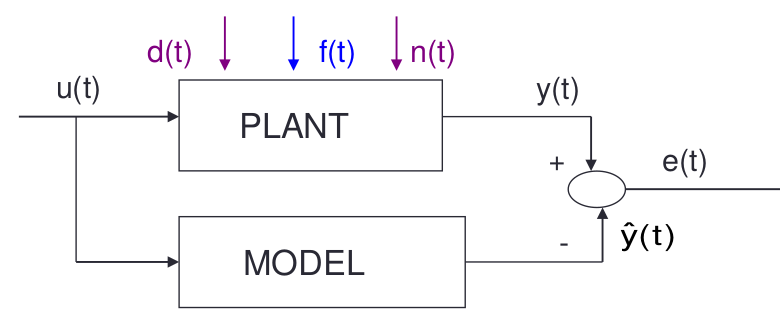
\includegraphics[width=0.9\linewidth]{model_based.png}
    \caption{Model-based fault detection}
    \label{fig:model_based}
\end{subfigure}%
\begin{subfigure}{0.5\textwidth}
    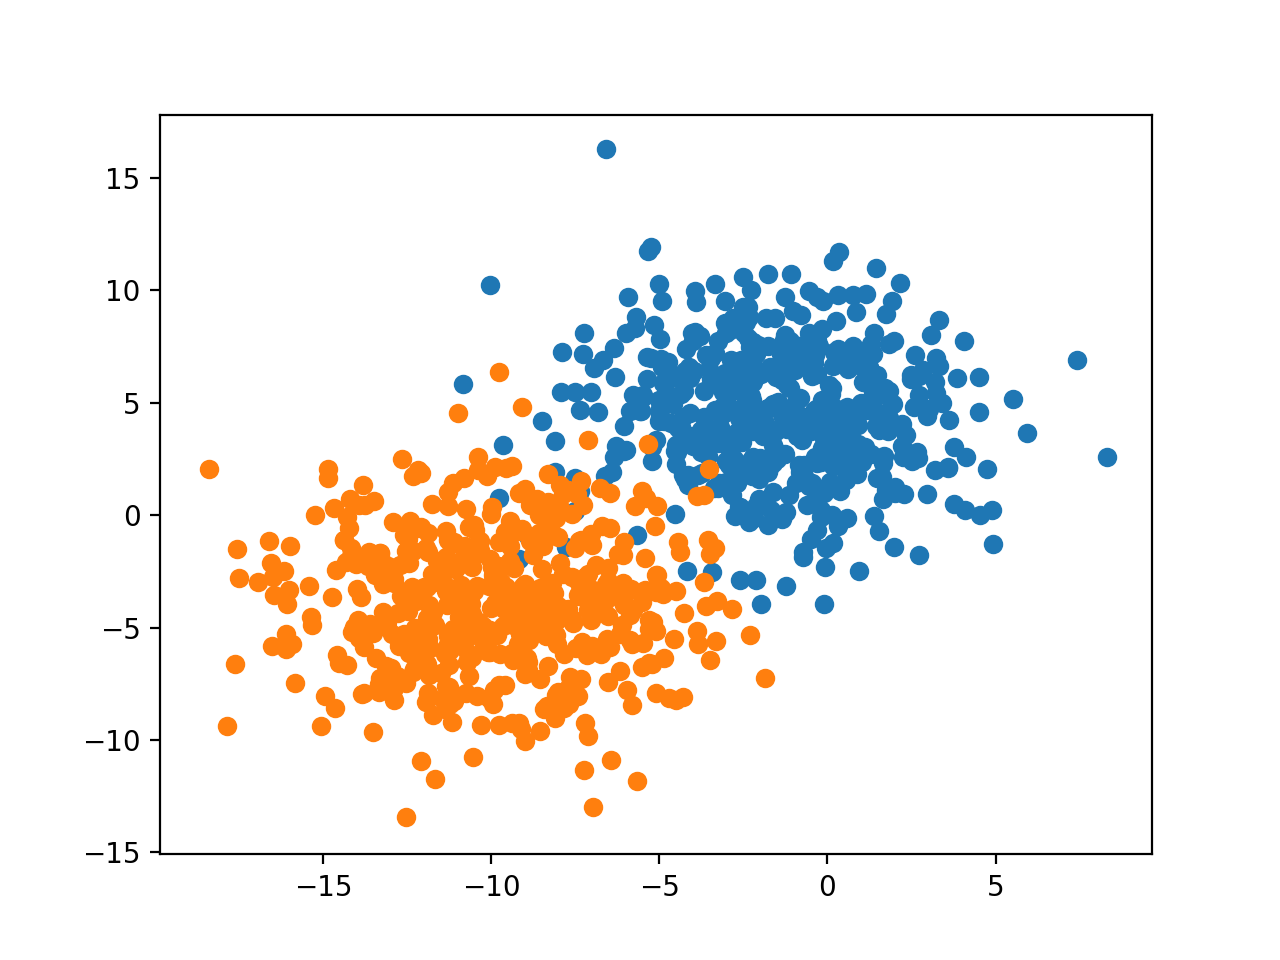
\includegraphics[width=0.9\linewidth]{signal_based.png}
    \caption{Signal-based fault detection}
    \label{fig:signal_based}
\end{subfigure}
\caption{Fault detection common approaches}
\label{fig:fault_detection}
\end{figure}

\subsubsection{Signal-Based methods}
\begin{itemize}
    \item Limit Checking and Trend Checking
    \item Data Analysis (PCA)
    \item Spectral Analysis
    \item Parametric Signal Models
    \item Pattern Recognition (kNN, ANN, SOM)
\end{itemize}
\subsubsection{Model-Based methods}
We know system structure. Faults modeled as some system variables changes.
Parameter estimation


\subsubsection{Knowledge-Based methods}


The result of FDI is the detection and identification of faults that occur
during the operation of the device. Subsequently data is processed using
Fault Tolerance and Predictive maintenance methods.

\textbf{Fault Tolerance}: Provide the system with the hardware architecture and
  software mechanisms which will allow, if possible to achieve a given
  objective not only in normal operation, but also in given fault
  situations.


\subsubsection{Condition Monitoring}
There is a optimization between technical and financial possibilities in a
specific situation.

FMECA (Failure Mode, Effect and Criticality Analysis) \\
FTA (Fault Tree Analysis) \\
RCA (Root Cause Analysis) \\


% -----------------------------------------------------------------------------
% 
% -----------------------------------------------------------------------------


\subsection{Predictive maintenance}
\textbf{Predictive maintenance (PdM)} is cost-effective maintenance strategy that
predicts time to failure and warns of an anticipated location where this
could occur.

\subsubsection{Goals}
The are two main goals of Predictive maintenance, RUL (remaining useful
life) estimation and identification where the future failure can appear, or what is
the reason of decreasing RUL. 
As a result of PM is RUL representing of number cycles, days, or some time
period before fault occurred. And probability where this fault can appear.

Predict where, when and what is the reason of failure (identify primary
factors).


\textbf{Predictive maintenance development sequence}:
\begin{enumerate}
    \item{Collect data (using sensors, math model)}
    \item{Process data (clean up data)}
    \item{Identify Condition Indicators CI}
        \begin{itemize}
            \item{Signal-based CI}
            \item{Model-based CI}
        \end{itemize}
    \item{Fit model (ML techniques)}
    \item{Deploy monitoring and integrate}
    \item{Dashboard (UI)}
\end{enumerate}


\subsubsection{Methods}
There are couples of signal processing and analyzing methods that used in
both PM and FDI. For example:

\paragraph{Signal-Based} approach is suitable in situation when we have
measurements from system in different operating conditions. 
But there is a problem that Signal-Based approach enable to classify and
learn patterns observed in training dataset. 


\paragraph{Model-Based} approach is to use physical failure models. This
models do not require a large dataset of failure data. And they can work in
situations never observed before. 


\begin{itemize}
    \item Spectral Analysis
    \item Wavelet Analysis
    \item Wavelet transform
    \item FFT
    \item Short Term Fourier Transform
    \item Gabor Expansion
    \item Wigner-Ville distribution
    \item Correlation
    \item High resolution spectral analysis
    \item Waveform Analysis
    \item Time-Frequency Analysis
    \item PCA
    \item Machine Learning techniques:
        \begin{itemize}
            \item kNN
            \item ANN
        \end{itemize}
\end{itemize}

\subsubsection{Using model of the system in PM}

Mathematical model of the real world system can be created using different
approaches. Modeling based on Physical modeling (Simscape) data-driven
modeling where system is represented as a "Black box" or some combination
of this approaches.
Model with estimated parameters uses for simulation system behavior in
different working conditions and with different faults during working
process.

Measured data, Generated data from mathematical model, or Synthetic data
(Combination of measured and generated) can be used for assessment of
Condition Indicators. 

Condition Indicators are features extracted from the signals, representing some
system behavior and hides some information about system processing.

Condition indicators represented by three main domain. There are Time
domain, Frequency domain, Time-Frequency domain Condition Indicators.

\subsubsection{Digital twin}

%\subsubsection{Detect and Diagnose Faults}
%Using condition indicators on Test data we can analyze actual system state.
%Designing algorithm is iterative process when you try different
%combinations of condition indicators and different models to evaluate best
%results.

\subsection{Comparison PM and FDA approaches}

\subsection{Application field}

\end{document}


\chapter{Demonstration Device Overview}

\section{Double-Acting Pneumatic Actuator}
\begin{figure}[h!]
    \centering
    \begin{subfigure}[b]{0.3\textwidth}
        \centering
        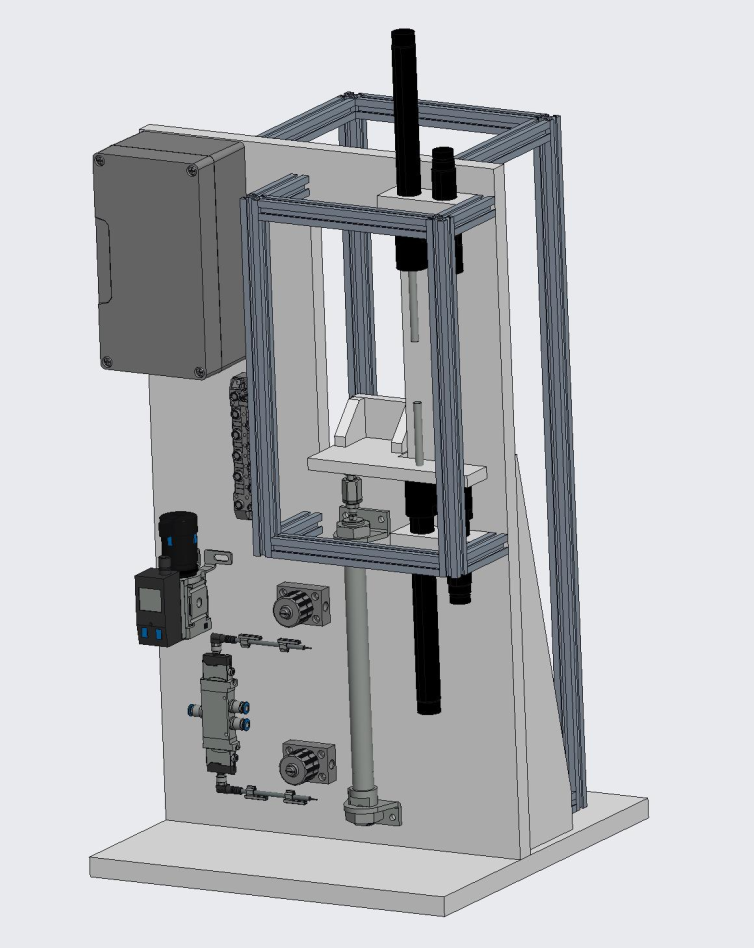
\includegraphics[width=1\textwidth]{model3d.png}
        \caption{3D render of the demonstration device}
        \label{fig:3d}
    \end{subfigure} 
    \hfill
    \begin{subfigure}[b]{0.6\textwidth}
        \centering
        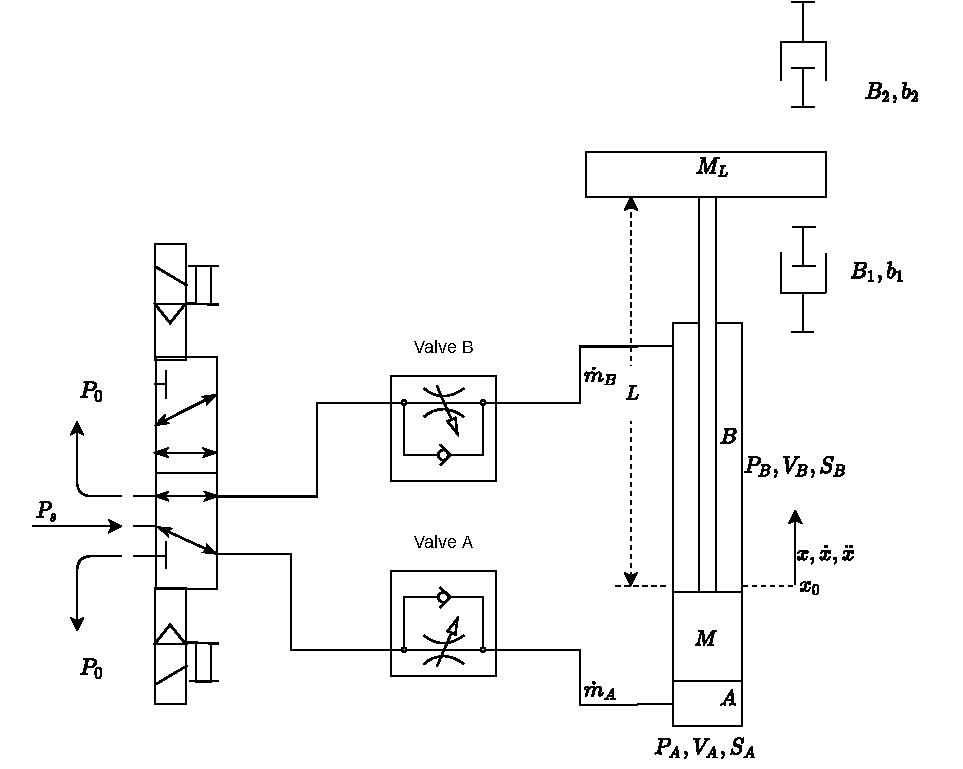
\includegraphics[width=1\textwidth]{system_scheme.pdf}
        \caption{Schematically representation of the demonstration device}
        \label{fig:device_scheme}
    \end{subfigure}
    \caption{Demonstration device}
    \label{fig:device}
\end{figure}

The case study of this thesis is the double-acting pneumatic piston, with a
pneumatic circuit and mechanical assembly driven by a piston.  Figure
\ref{fig:device_scheme} is a schematical representation of the system.
Figure \ref{fig:3d} is a 3D render of the system.

Pneumatic systems use air to transmit power between components in the
circuit. The air is a compressible gas, and we have to consider this when
designing a model. Pneumatic actuators are highly efficient and fast
drives. Using compressed air pneumatic actuator can move with high
velocities and supply nominal force in the kN range. One of the advantages
of a pneumatic system with a piston is that only one supply line is
necessary, giving many opportunities to design and maintain the system.
The basic pneumatic system includes an air reservoir with supplied air,
pressure lines connection, pneumatic actuator and control valve to connect
the supply pressure and actuator. Resistance to movement places a mass that
acts on the piston. 

In this thesis, a double-acting pneumatic actuator, as shown in figure
\ref{fig:device_scheme} was used. Throttling valves A and B regulate the air mass flow to
the piston's chambers. Proportion valve connects supply and ambient
pressure lines to achieve piston control. There are two pairs of dampers
installed to prevent possible destruction impact and simulate different
material penetration resistance.

The demonstration device can be used in stamping, drilling, moving
applications.

\section{Sensors}

There are eight types of sensors located on the system. Table
\ref{tab:sensors_tab} describes a sensor purpose, signal name in the
datastore, and the signal unit. 

\begin{table}[h!]
    \centering
    \begin{tabular}{|c|c|c|c|}
\hline
\textbf{Sensor} & \textbf{Unit} & \textbf{Description} & \textbf{Name} \\
\hline
Encoder       & m     & displacement                           & LeverPosition \\
Encoder       & m/s   & velocity                               & LeverVelocity \\
Accelerometer & g     & accelerometer on moving part           & AccelerometerMovin\_axisZ/Y \\ 
Accelerometer & g     & accelerometer on static part           & AccelerometerStatic\_axisZ/Y \\ 
Flow Sensor   & l/min & air flow extrusion to A chamber        & FlowExtrusion \\
Flow Sensor   & l/min & air flow contraction from A chamber    & FlowContraction \\
Pressure      & bar   & pressure measurement in reservoir      & AirPressure \\
Microphone    & V     & microphone on upper bumper             & MIC\_uBumper \\ 
Microphone    & V     & microphone on bottom bumper            & MIC\_bBumper \\ 
Microphone    & V     & ambient microphone                     & MIC\_Ambient \\
Temperature   & $^o$C & cylinder temperature measurement       & TempCylinder \\
Temperature   & $^o$C & ambient temperature measurement        & TempAmbient \\
Strain Gauge  & Pa    & strain measurements                    & StrainGauge \\
Proximity     & -     & upper bound detection                  & ProximitySensor_upper \\
Proximity     & -     & bottom bound detection                 & ProximitySensor_bottom \\
\hline
    \end{tabular}
    \caption{Sensors overview}
    \label{tab:sensors_tab}
\end{table}

The dataset measured on the system contains almost five thousand
measurements in different operating conditions. Each measurement includes a
10-second recording of moving the pistol up and down. This data was given
in the format of massive files with the ".mat" extension, which was divided
into files contains only one measurement.  The divided dataset is easier to
maintain, and Matlab recommends this type of datastores called Data
Ensemble \ref{}.

The measured examples are shown in figures
\ref{fig:over_examp_1},\ref{fig:over_examp_3}, and \ref{fig:over_examp_3}.

\begin{figure}[!htb]
    \centering
    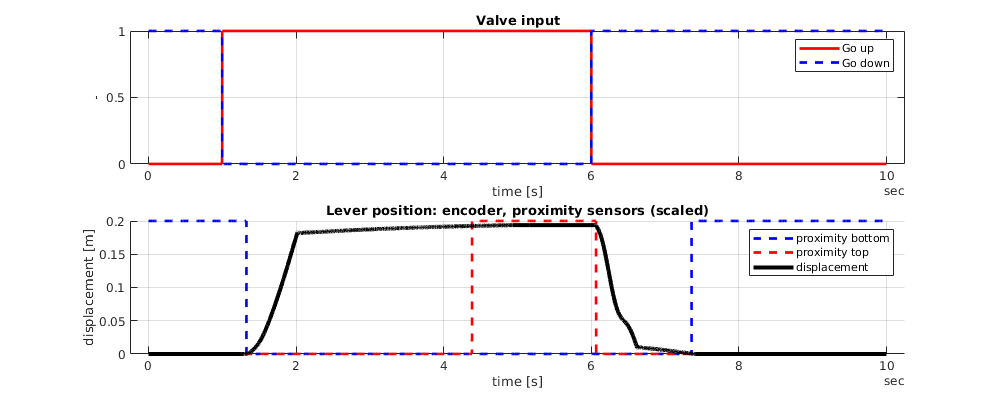
\includegraphics[width=1\textwidth]{overview_data_example_4.png}
    \caption{Caption}
    \label{fig:over_examp_1}
\end{figure}


\newpage
\begin{figure}[!htb]
    \centering
    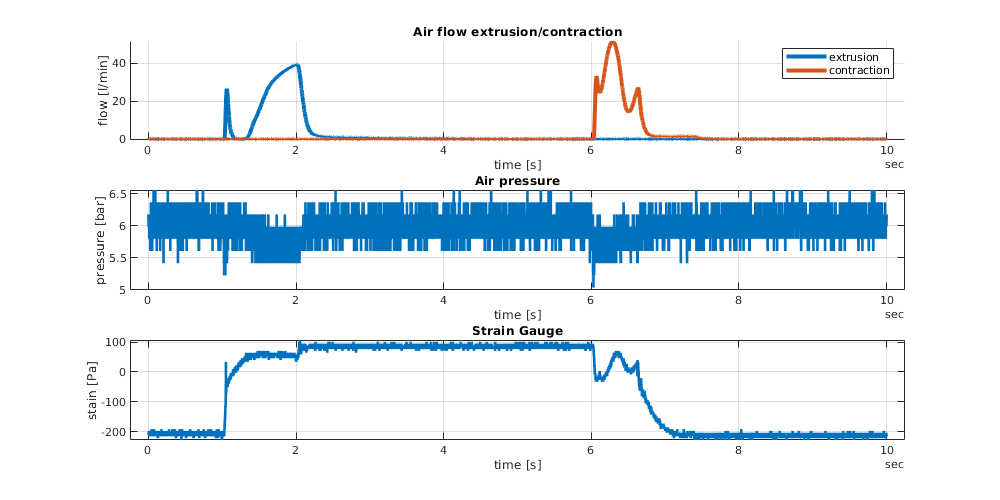
\includegraphics[width=1\textwidth]{overview_data_example_1.png}
    \caption{Caption}
    \label{fig:over_examp_2}
\end{figure}

\begin{figure}[!htb]
    \centering
    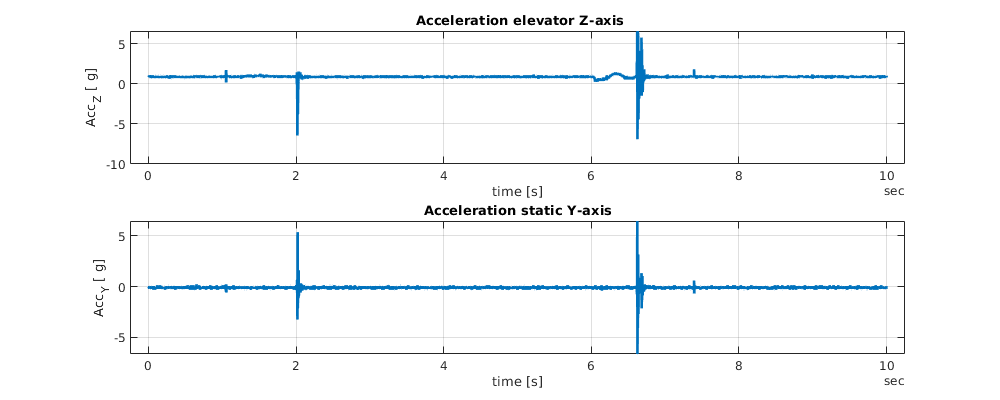
\includegraphics[width=1\textwidth]{overview_data_example_2.png}
    \caption{Caption}
    \label{fig:over_examp_3}
\end{figure}

%\begin{figure}[!htb]
%    \centering
%    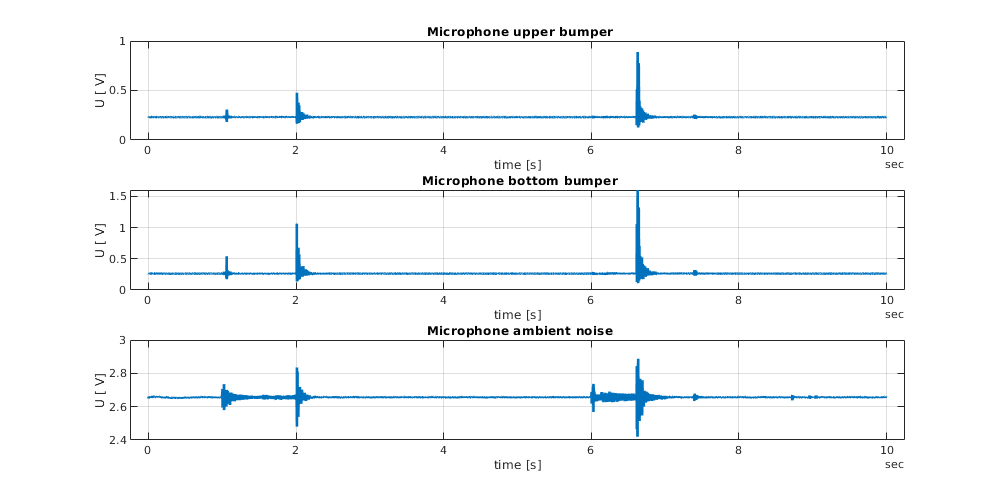
\includegraphics[width=1\textwidth]{overview_data_example_3.png}
%    \caption{Caption}
%    \label{fig:over_examp_4}
%\end{figure}

TODO text




% Artyom Voronin
%  __  __           _      _ 
% |  \/  | ___   __| | ___| |
% | |\/| |/ _ \ / _` |/ _ \ |
% | |  | | (_) | (_| |  __/ |
% |_|  |_|\___/ \__,_|\___|_|
%                            
% Brno, 2020

\documentclass[class=article, crop=false]{standalone}
\usepackage[subpreambles=true]{standalone}

\usepackage{subcaption}
\usepackage{caption}
\usepackage{sectsty}
\usepackage{graphicx}
\graphicspath{{img/}{../img/}{../../img/}}
\usepackage{listings}
\lstset{language=Python}
\usepackage{hyperref}
\usepackage{amsmath}
\usepackage{import}
\usepackage{subfiles}
\usepackage[utf8]{inputenc}
\usepackage[english]{babel}

%\usepackage[square, numbers]{natbib}
%\bibliographystyle{unsrtnat}
%\usepackage[nottoc]{tocbibind}

%\usepackage{biblatex}
%\addbibresource{citations.bib} %usage \cite{test}
% Margins
% 
\topmargin=-0.45in
\evensidemargin=0in
\oddsidemargin=0in
\textwidth=6.5in
\textheight=9.0in
\headsep=0.25in

%\title{Models}
%\author{Artyom Voronin} 
%\date{}

\begin{document}
%\tableofcontents

% -------------------------------------------------------
% Section
% -------------------------------------------------------
\section{System modeling}

\paragraph{First Principles} (White-Box) \\
% TODO Isermann Fault Detection str 72
Simplification, Liniarization, Reduction, Parameter Estimation. \\
SimScape (Physical modeling), Simulink (Differential equations).

\paragraph{Data-Driven modeling}(Black-Box) \\ % In many cases better for prediction
% TODO Isermann Fault Detection str 72
Measurements, Identification.

% Nonlinear dynamic modeling  Isermann FDS str. 84

\subsection{Pneumatic piston system overview}
%\begin{figure}[h!]
%    \centering
%    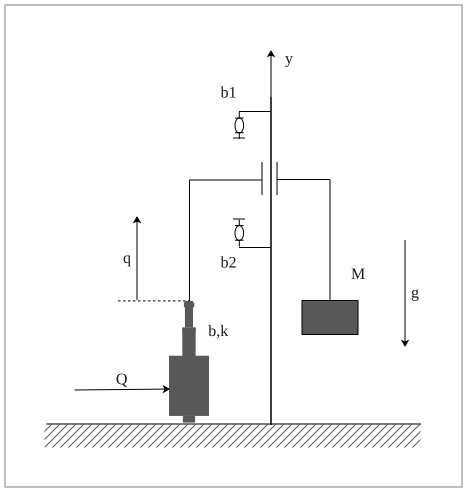
\includegraphics[width=0.5\textwidth]{model_draw_vec.png}
%    \caption{Schematic model}
%    \label{fig:model_draw}
%\end{figure}


% -------------------------------------------------------
% 
% -------------------------------------------------------

\subsection{Mechanical assembly}
\subsubsection{Equation of motion}

The motion of the pneumatic piston mechanism describes in terms of the
general 1dof dynamical equation \ref{eq:1dof}. 

\begin{equation}
    m\ddot{x} + b\dot{x} + kx = u
    \label{eq:1dof}
\end{equation}

%\begin{equation*}
%    \ddot{x} +\frac{b}{m}\dot{x} + \frac{k}{m}x = \frac{1}{m}u
%\end{equation*}
%
%\begin{equation*}
%    \ddot{x} +2\delta\dot{x} + \Omega^2x = \frac{1}{m}u
%\end{equation*}
%
%where $\delta = \frac{b}{2m}$ is damping and $\Omega = \sqrt{\frac{k}{m}}$
%is natural frequency of system.
%\begin{equation*}
%    \ddot{x} +2\zeta\Omega\dot{x} + \Omega^2x = \frac{1}{m}u
%\end{equation*}
%where $\zeta = \frac{b}{2\sqrt{km}}$ is damping ratio.


In the case of the pneumatic piston, the equation \ref{eq:1dof}
transforms into an equation \ref{eq:mechanical}.

\begin{equation}
    (M + M_L) \ddot{x} + F_{damp} + F_g + F_{hs}  = F_p
    \label{eq:mechanical}
\end{equation}

Where $M$ represents a mass of the all moveable part of the piston,
$M_L$ is load mass, $F_g$ gravity force acting to mechanical moving assembly,
$F_{hs}$ - models endpoints (hard stop),
$F_{damp}$ represents shock absorbers acted at endpoints,
$F_{p}$ is a force produced by the pneumatic piston \ref{eq:pneum}.

\begin{equation}
    F_p = P_A S_A - P_B S_B - P_0 S_0
    \label{eq:pneum}
\end{equation}

\subsubsection{Hard stop}
Hard stop can be represented as spring and dumps:

\begin{align}
    F_{HS} =
    \begin{cases}
        K_p(x-g_p) + D_pv & \text{for } x \ge g_p \\
        0 & \text{for } g_n < x < g_p \\
        K_n(x-g_n) + D_nv & \text{for } x \le g_n \\
    \end{cases}
\end{align}


Possible parameters: \\
\begin{tabular}{ |c|c|c| }
    \hline
    $K_p$ & $10^6$ & $[kg/s^2]$  \\
    $K_n$ & $10^6$ & $[kg/s^2]$  \\
    $D_p$ & $350$  & $[kg/s]$    \\
    $D_n$ & $350$  & $[kg/s]$    \\
    $g_n$ & $0  $  & $[m]$       \\
    $g_p$ & $0.2$  & $[m]$       \\
    \hline
\end{tabular}

\subsubsection{Shock Absorbers}

\subsection{Pressure model}

\begin{tabular}{ |c|c|c| }
    \hline
    $p_A, p_B$              & $Pa$              & pressure in chamber A, B \\
    $\dot{m_A}, \dot{m_B}$  & $kg \cdot s^{-1}$ & mass flow on way to chamber A, B \\
    $S_A, S_B$              & $m^2$             & piston area  \\
    $V_A, V_B$              & $m^3$             & volume of chamber A,B \\
    $V_{0A}, V_{0B}$        & $m^3$             & "dead" volume of chamber A,B \\
    $m$                     & $kg$              & piston mass\\
    $F_{load}$              & $N$               & load \\
    $x$                     & $m$               & piston position \\
    $l$                     & $m$               & maximum piston position \\
    \hline
\end{tabular}



\paragraph{Isothermal model}
\begin{align}
    m = \rho V \\
    \dot{m} = \dot{\rho} V + \rho \dot{V}
\end{align}

Applying \ref{eq:equation_of_state}:
\begin{align}
    \rho = \frac{p}{RT} \\
    \dot{\rho} = \frac{\dot{p}}{RT} 
\end{align}

Finally get \ref{eq:pressure1}:
\begin{align}
    \dot{p} = - \frac{p}{V}\dot{V} + \frac{RT}{V}\dot{m}
    \label{eq:pressure1}
\end{align}

\paragraph{Adiabatic model} 
For simple adiabatic model following equation can be used
\ref{eq:pressure_adiabatic_simple_model}:

\begin{align}
    \dot{p} = - \frac{\gamma p}{V}\dot{V} + \frac{\gamma RT}{V}\dot{m}
    \label{eq:pressure_adiabatic_simple_model}
\end{align}

\begin{align}
    \dot{p_A} = \frac{\gamma}{S_A x + V_{0A}} \left(- p_A S_A\dot{x} + RT_A\dot{m_A}
    \right)
\end{align}

\begin{align}
    \dot{p_B} = \frac{\gamma}{S_B (l-x) + V_{0B}} \left(p_B S_B\dot{x} + RT_B\dot{m_B}
    \right)
\end{align}

Volumes of chambers:
\begin{align}
    V_A = S_A x + V_{0A} \\
    V_B = S_B (l-x) + V_{0B} \\
    \dot{V}_A = S_A \dot{x} \\
    \dot{V}_B = - S_B \dot{x}
\end{align}

$T_A, T_B$ calculated from \ref{eq:equation_of_state}, or in adiabatic
model this parameters can remain constant same as atmospheric temperature.




\subsection{General physical principles}

\subsubsection{Thermodynamics}
\begin{tabular}{ |c|c|c| }
    \hline
    $p$                     & $Pa$              & pressure \\
    $V$                     & $m^3$             & volume \\
    $m$                     & $kg$              & mass \\
    $n$                     & $mol$             & amount of substance \\
    $R$                     & $Jkg^{-1}K^{-1}$  & ideal gas constant \\
    $r$                     & $Jkg^{-1}K^{-1}$  & mass-specific gas constant \\
    $T$                     & $K$               & temperature \\
    $S$                     & $m$               & area \\
    $z$                     & $m$               & height \\
    $w$                     & $ms^{-1}$         & flow speed \\
    $H$                     & $J$               & enthalpy \\
    $\nu$                   & $m^3kg^{-1}$      & specific volume \\
    $Q$                     & $J$               & heat shared with
                                                    environment \\
    $W_T$                   & $J$               & work \\
    $c_p$                   & $Jkg^{-1}K^{-1}$  & is the specific heat
                                                    at constant pressure \\
    $c_v$                   & $Jkg^{-1}K^{-1}$  & is the specific heat at constant volume\\
    $g=9.81$                & $ms^{-2}$         & gravity acceleration \\
    $\gamma=1.4\text{(air)}$& $-$               & heat capacity ratio
                                                    (isentropic expansion factor)\\
    \hline
\end{tabular}

\subsubsection{Equation of state}
Generally $pV=nRT$ but for air purpose were $r=\frac{pv}{T}=R=287.1 [Jkg^{-1}K^{-1}]$
following equation can be used \ref{eq:equation_of_state}:
\begin{align}
    pV = mrT
    \label{eq:equation_of_state}
\end{align} 

\subsubsection{Isothermal process}
Used in some papers \ref{eq:isothermal_process}:
\begin{align}
    p_1 V_1 = p_2 V_2 = const
    \label{eq:isothermal_process}
\end{align}
\subsubsection{Adiabatic process}

Adiabatic process \ref{eq:adiobatic_process}:
\begin{align}
     p_1V_1^{\gamma} =  p_2V_2^{\gamma} = const
    \label{eq:adiobatic_process}
\end{align}

Heat capacity ratio:
\begin{align}
    \gamma = \frac{c_p}{c_v}
\end{align}

Mayer's relation:
\begin{align}
    c_p = c_v + R
\end{align}

\subsubsection{Bernoulli's principle}
Bernoulli's principle \ref{eq:bernoullis_principle}:
\begin{align}
    H_1 + \frac{mw_1^2}{2} + mgz_1 + Q = H_2 + \frac{mw_2^2}{2} + mgz_w +
    W_T
    \label{eq:bernoullis_principle}
\end{align}

\begin{align}
    H_1- H_2 = -\int_1^2 V dp = c_p(T_1-T_2) = c_p T_1(1-\frac{T_2}{T_1})
    \label{eq:etalpi_sub}
\end{align}

Differential form:
\begin{align}
    \nu dp + w dw + g dz + dw_T = 0
\end{align}


\subsubsection{Fluid mechanics}
\begin{tabular}{ |c|c|c| }
    \hline
    $\dot{m}$                   & $kgs^{-1}$  & mass flow \\
    $c$                         & $ms^{-2}$   & speed of sound \\
    $w_k$                       & $ms^{-2}$   & critical flow velocity \\
    $\psi$                      & $-$         & flow coefficient \\
    $\psi_{max}$                & $-$         & critical flow coefficient \\
    $\beta$                     & $-$         & ration of pressure
                                                    differential \\
    $\beta_k$                   & $-$         & critical ratio of pressure
                                                    differential \\

    \hline
\end{tabular}

Continuity equation \ref{eq:continuity_equation}: 
\begin{align}
    \dot{m} = S_1 w_1 \rho_1 = S_2 w_2 \rho_2 = const
    \label{eq:continuity_equation}
\end{align}

\subsubsection{Air expansion from tank}
Assuming $W_T = 0, z_1 = z_2, Q = 0$ conditions and combine with
\ref{eq:bernoullis_principle} we will get \ref{eq:w2} equation:

\begin{align}
    w_2 = \sqrt{2(H_1 - H_2)}
    \label{eq:w2}
\end{align}

\begin{align}
    w_2 =
    \sqrt{2RT_1(\frac{\gamma}{\gamma-1})(1-(\frac{p_2}{p_1})^\frac{\gamma-1}{\gamma})}
    \label{eq:w2_final}
\end{align}

\begin{align}
    \rho_2 = \frac{p_1}{RT_1} (\frac{p_2}{p_1})^{\frac{1}{\gamma}}
    \label{eq:rho2}
\end{align}

Together \ref{eq:continuity_equation} \ref{eq:w2_final} \ref{eq:rho2}:
\begin{align}
    \dot{m} = S p_1 \sqrt{\frac{2}{RT_1}} \cdot
    \sqrt{\frac{\gamma}{\gamma-1}\left(\left(\frac{p_2}{p_1}\right)^\frac{2}{\gamma} -
    \left(\frac{p_2}{p_1}\right)^\frac{\gamma + 1}{\gamma}\right)}
    \label{}
\end{align}

where: 
\begin{align}
    \psi\left(\frac{p_2}{p_1}\right) =  
    \sqrt{\frac{\gamma}{\gamma-1}\left(\left(\frac{p_2}{p_1}\right)^\frac{2}{\gamma} -
    \left(\frac{p_2}{p_1}\right)^\frac{\gamma + 1}{\gamma}\right)}
    \label{eq:psi}
\end{align}

Finally \ref{eq:mass_flow}:
\begin{align}
    \dot{m} = Sp_1\sqrt{\frac{2}{RT_1}} \psi\left(\frac{p_2}{p_1}\right)
    \label{eq:mass_flow}
\end{align}

\subsubsection{Critical flow velocity}
Speed of sound:
\begin{align}
    c = \sqrt{\frac{dp}{d\rho}} = 
    \sqrt{\frac{\gamma p}{\rho}} = \sqrt{\gamma R T}
    \label{eq:speed_of_sound}
\end{align}

Assume $c=w_2$ (\ref{eq:w2_final}, \ref{eq:speed_of_sound}) we will get the
critical flow velocity:
\begin{align}
    &c_2 = w_k = \sqrt{\gamma RT} =
    \sqrt{2RT_1\frac{\gamma}{\gamma-1}-2w_k^2\frac{1}{\gamma-1}} \\
    &w_k^2 = 2RT_1\frac{\gamma}{\gamma-1}-2w_k^2\frac{1}{\gamma-1} \\
    &w_k = \sqrt{2RT_1\frac{\gamma}{\gamma-1}} = \sqrt{2p_1 \nu_1 \frac{\gamma}{\gamma + 1}}
    \label{eq:wk}
\end{align}


For calculating critical pressure ratio assume $w_k = w_2$ \ref{eq:wk}
\ref{eq:w2_final}:
\begin{align}
    &\sqrt{2RT_1\frac{\gamma}{\gamma-1}}  = 
    \sqrt{2RT_1 \frac{\gamma}{\gamma-1}
    \left(1-\left(\frac{p_2}{p1}\right)^{\frac{\gamma+1}{\gamma}}\right)} \\
    &\left(\frac{p_2}{p1}\right)^\frac{\gamma-1}{\gamma} = \frac{2}{\gamma+1} \\
\end{align}
\begin{align}
    &\left(\frac{p_2}{p1}\right)_k =
    \left(\frac{p_k}{p1}\right) =
    \left(\frac{2}{\gamma+1}\right)^\frac{\gamma}{\gamma-1}=\beta_k
    \label{eq:beta_k}
\end{align}

Critical pressure condition is $p_k = p_1 \beta_k$.

Applying \ref{eq:beta_k} to \ref{eq:psi}:
\begin{align}
    &\psi_{max} (\beta_k) = 
    \left(\frac{2}{\gamma+1}\right)^\frac{\gamma}{\gamma-1}\sqrt{\frac{\gamma}{\gamma+1}}
\end{align}

For air $\beta_k = 0.528, \psi_{max} = 0.484$


Final equation for $\psi$:
\begin{align}
    \psi\left(\frac{p_2}{p_1}\right) = 
    \begin{cases}
    \sqrt{\frac{\gamma}{\gamma-1}\left(\left(\frac{p_2}{p_1}\right)^\frac{2}{\gamma} -
    \left(\frac{p_2}{p_1}\right)^\frac{\gamma + 1}{\gamma}\right)} & 0.528
    <\frac{p_2}{p_1} \le 1 \\
    \left(\frac{2}{\gamma +1}\right)^{\frac{1}{\gamma+1}}
    \sqrt{\frac{\gamma}{\gamma +1}} & 0 \ge \frac{p2}{p1} \le 0.528\\
    \end{cases}
\end{align}



\subsection{Pneumatic actuator model}

\subsubsection{Input/Output mass flows}

\begin{align}
    \dot{m}T = \dot{m_{in}}T_s - \dot{m_{out}}T_{A/B}
\end{align}


\subsubsection{Differential equation for Temperature change}
\begin{align}
    T = \int{ (\gamma T_s - T_{A/B})
        \frac{R\dot{m}_{A/Bin}}{p_{A/B}V_{A}}T_{A/B} -
    (\gamma-1)\frac{R\dot{m}_{A/Bout}}{p_{A/B}V_{A/B}} T_{A/B}^2 -
(\gamma-1)\frac{\dot{V}_{A/B}}{V_{A/B}}T_{A/B}}
\end{align}


\subsubsection{Valve model} %TODO
\begin{tabular}{ |c|c|c| }
    \hline
    $S_{eq}$                & $m^2$         & Equivalent cross section \\
    $S_{max}$               & $m^2$         & Maximum cross section \\
    $Cd$                    & $-$           & Coefficient of contraction \\
    $u$                     & $-$           & Regulation variable \\
    \hline
\end{tabular}

\paragraph{Valve flow model with simply input control signal}
For regulation flow this model used input control signal directly without
spool mechanics.

Coefficient of contraction \ref{eq:coefficient_of_contraction}:
\begin{align}
    C_d = \frac{S_{eq}}{S_{max}}
    \label{eq:coefficient_of_contraction}
\end{align}

For flow control regulation $u \in \langle-1,1\rangle$ can be used.
\begin{align}
    u =
    \begin{cases}
        u \in \langle -1, 0) & \text{discharge the chamber} \\
        u = 0& \text{valve closed}  \\
        u \in (0, 1\rangle & \text{filling the chamber} 
    \end{cases}
\end{align} 

\begin{align}
    \dot{m} = u S_{max} C_d p_1 \sqrt{\frac{2}{RT_1}}
    \cdot \psi\left(\frac{p_2}{p_1}\right)
    \label{eq:flow}
\end{align}

\textbf{For filling the chamber:}
\begin{itemize}
\item $p_1 = p_s$ 
\item $p_2 = p_A \text{ or } p_B$
\item $T_1 = T_s$
\end{itemize}

\textbf{For discharge the chamber:}
\begin{itemize}
\item $p_1 = p_A \text{ or } p_B$
\item $p_2 = p_0$
\item $T_1 = T_A, T_B$
\end{itemize}

where $p_s$ is supply pressure. $p_0$ atmospheric pressure. As $T_i$ - 
atmospheric temperature using according to isothermal process.

\begin{align}
    \dot{m}_A =
    \begin{cases}
        u S_v C_d p_s \sqrt{\frac{2}{RT_s}}
        \cdot \psi\left(\frac{p_A}{p_s}\right)  &,   u \in (0, 1 \rangle \\
        0   &,  u = 0 \\
        u S_v C_d p_A \sqrt{\frac{2}{RT_A}}
        \cdot \psi\left(\frac{p_0}{p_A}\right)  &,   u \in \langle -1, 0) \\
    \end{cases}
\end{align}

\begin{align}
    \dot{m}_B =
    \begin{cases}
        u S_v C_d p_s \sqrt{\frac{2}{RT_s}}
        \cdot \psi\left(\frac{p_B}{p_s}\right)  &,   u \in (0, 1 \rangle \\
        0   &,  u = 0 \\
        u S_v C_d p_A \sqrt{\frac{2}{RT_B}}
        \cdot \psi\left(\frac{p_0}{p_B}\right)  &,   u \in \langle -1, 0) \\
    \end{cases}
\end{align}

\paragraph{Valve flow with spool mechanic included}

With respect to valve spool modeled as 1DOF system \ref{eq:1dof} and
mechanical and geometrical properties following equation were used.

\paragraph{Valve flow with spool}
In this model we accept a spool displacement $x_s$, controlled by input
voltage $u$.

\begin{equation}
    \dot{m}(P_u, P_d) = 
    \begin{cases}
        C_f A_v
        \left(\frac{\gamma}{R}\left(\frac{2}{\gamma-1}\right)\right)^{\frac{1}{2}}
        \cdot
        \frac{P_u}{\sqrt{T}}\left(\frac{P_d}{P_u}\right)^{\frac{1}{\gamma}}
        \cdot 
        \sqrt{1 - \left(\frac{P_d}{P_u}\right)^{\frac{\gamma-1}{\gamma}}} &,
            \text{ if } \frac{P_d}{P_u}>P_{cr} \text{ (subsonic)} \\
        C_f A_v \frac{P_u}{\sqrt{T}}\cdot \sqrt{\frac{\gamma}{R}
        \left(\frac{2}{\gamma + 1}\right)^{\frac{\gamma+1}{\gamma-1}}} &,
            \text{ if }  \frac{P_d}{P_u} \le P_{cr} \text{ (sonic)} \\
    \end{cases}
    \label{eq:valve_2}
\end{equation}

where $C_f$ is discharge coefficient, $A_v$ is the effective are of valve
orifice.

\begin{equation}
    A_v = \frac{\pi x_s^2}{4}
    \label{eq:A_v}
\end{equation}

\begin{equation}
    x_s = C_v u
    \label{eq:x_s}
\end{equation}

where $C_v$ is the valve constant.

\paragraph{Valve model by Endler}
Require fitting constants and generally system identification.
Mass flow rates are given by following equations:


\begin{equation}
    \begin{aligned}
        \dot{m}_A(u, p_A) = g_1(p_A, sign(u))arctg(2u) \\
        \dot{m}_B(u, p_B) = g_2(p_B, sign(u))arctg(2u)
    \end{aligned}
\end{equation}

where $g_1, g_2$ are signal functions given:
\begin{equation}
    \begin{aligned}
        g_1(p_A, sign(u)) = \beta \Delta p_A = 
        \begin{cases}
            (p_s - p_A) \beta^{ench} &, \rm \ if\  u \ge 0 \\
            (p_A - p_0) \beta^{esv} &, \rm \ if\  u  < 0 \\
        \end{cases} \\
        g_2(p_B, sign(u)) = \beta \Delta p_B = 
        \begin{cases}
            (p_s - p_B) \beta^{ench} &, \rm \ if\  u < 0 \\
            (p_B - p_0) \beta^{esv} &, \rm \ if\  u \ge 0 \\
        \end{cases}
    \end{aligned}
    \label{eq:valve_3}
\end{equation}

where $\beta^{ench}, \beta^{evs}$ are constant coefficients.
For fitting model stop piston (speed of piston is null). This mean that
volume is constant. We can measure flow rate $\dot{m}$ versus input voltage
$u$ with given pressure difference.

\paragraph{Valve dead-zone}
For more precision control and modeling of the valve system, valve
dead-zone can be used \ref{eq:deadzone}.

\begin{equation}
    u_z = 
    \begin{cases}
        g_z(u) < 0 &, \text{ if } u \le u_n \\
        0          &, \text{ if } u_n < u < u_p \\
        h_z(u) > 0 &, \text{ if } u \ge u_p \\
    \end{cases}  
    \label{eq:deadzone}
\end{equation}

\subsection{Mechanical assembly}\label{sec:mech_assembly}
Mechanical assembly basically represented by following equation
\ref{eq:mech}.

\begin{equation}
    \ddot{x} = \frac{1}{m}\left(S_A p_A - S_B p_B - S_0 p_0 - F_f \right)
    \label{eq:mech}
\end{equation}

where $F_f$ is a friction force. Friction force can be modeled in the
different ways.

As an example of possible model is following equation. That consist from
complex friction forces including viscous friction and Coulomb friction
\ref{eq:friction1}.
\begin{equation}
    F_f = 
    \begin{cases}
        C \dot{x} + \left(f_c + (f_s-f_c)
        e^{-\left(\frac{\dot{x}}{v_s}\right)^{\delta}}\right) sign(\dot{x}) &,
        \text{ if } \dot{x} \le v_e \\
        \mu \dot{x} &,
        \text{ if } \dot{x} > v_e \\
    \end{cases}
    \label{eq:friction1}
\end{equation}
where $C$ - viscous friction coefficient, $f_c$ - Coulomb friction, $f_s$ -
maximum static friction, $\mu$ - dynamic friction factor, $v_s$ - Stribeck velocity,
$\delta$ - arbitrary index, $v_e$ critical velocity.



\section{Models based on approximation}
Generally with dataset of input-output signals approximation model can be
fit. Using System Identification Toolbox and modeled as Black-Box or
Gray-Box models. This section attempted to fit some models using data from
SimScape and Equation model presented before.

Fit approximation model make sense only if we know what to fit. Using
signal process techniques and identify dominant signals that providing best
classification features we will train models with respect to this signals.

Demonstration scripts are done and waiting for signals :)

\subsection{State-space model}
\subsection{ARX model}

\pagebreak
\section{Models comparison}

\subsection{Model based on equations}
This model \ref{fig:model_equations} was developed with respect to equations represented in previous
section.

\begin{figure}[h!]
    \centering
    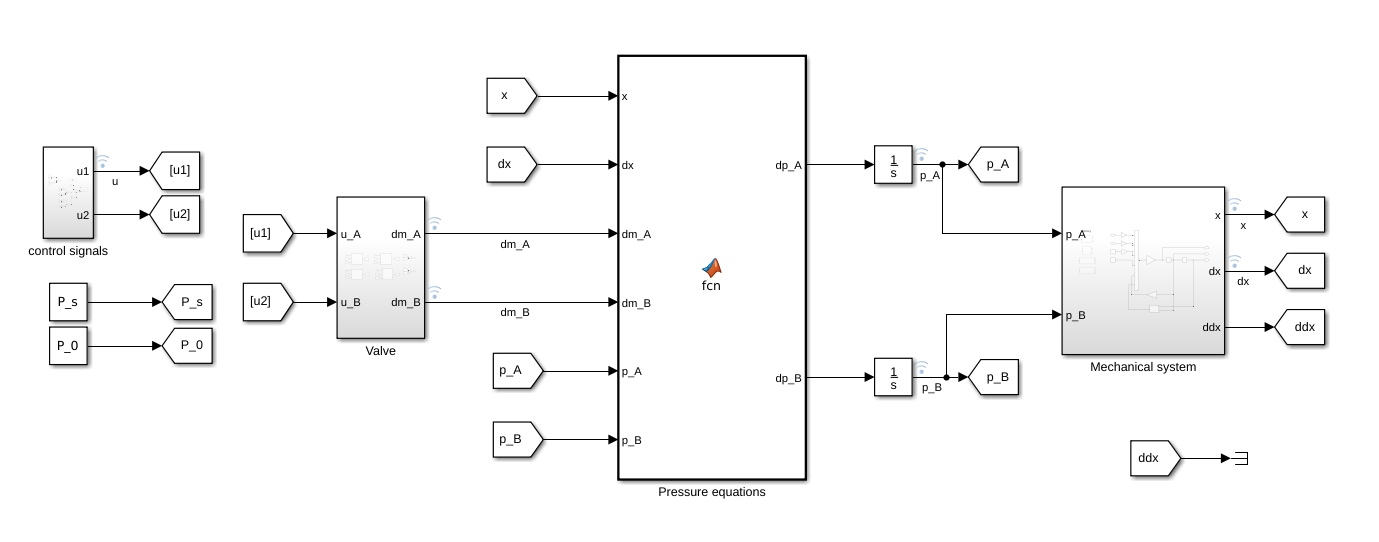
\includegraphics[width=1\textwidth]{equations.png}
    \caption{Simulink model based on equations}
    \label{fig:model_equations}
\end{figure}


\subsection{Model Simscape}
Model \ref{fig:model_simscape} was developed using SimScape toolbox.

\begin{figure}[h!]
    \centering
    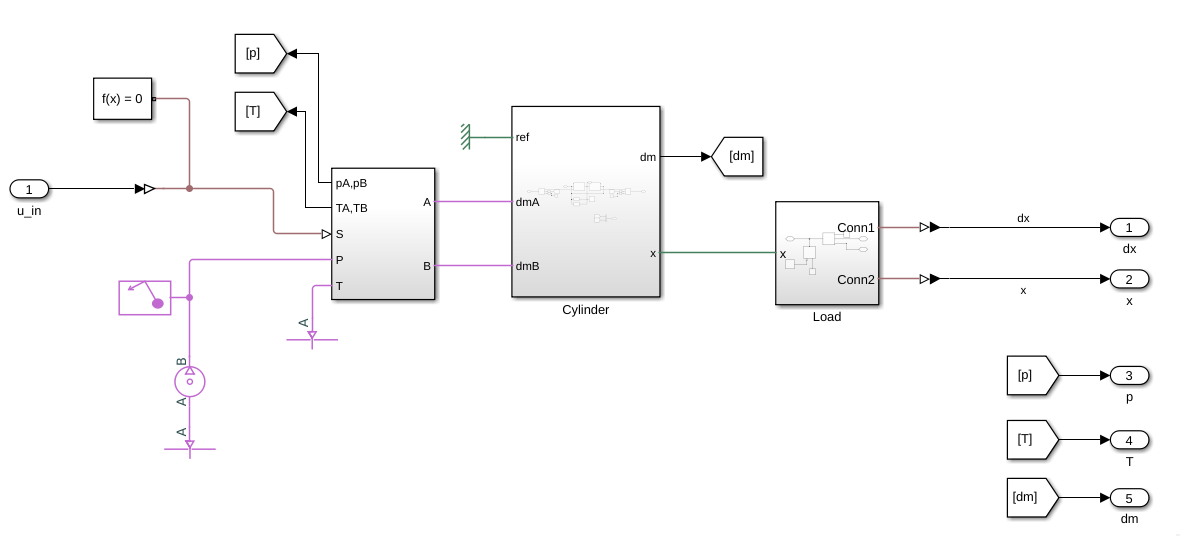
\includegraphics[width=1\textwidth]{simscape.png}
    \caption{Simulink model using SimScape Toolbox}
    \label{fig:model_simscape}
\end{figure}


\subsection{Comparison}
Following figure \ref{fig:compare_of_models} represent comparison of 2 models
(Simscape and based on equations) using same parameters for simulation:
There is slight difference between models causing Valve dynamics
simplifications in model based on equations.

\begin{figure}[h!]
    \centering
    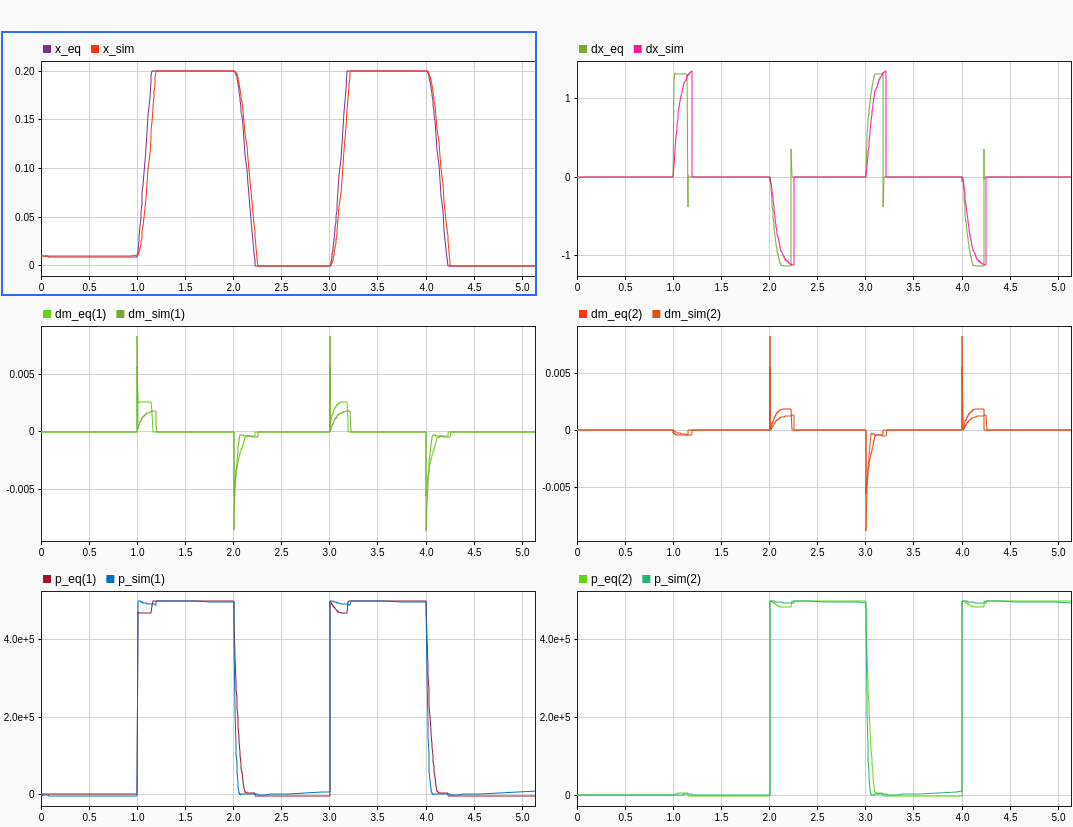
\includegraphics[width=1\textwidth]{models_comparation.png}
    \caption{Comparison of simscape and model based on equations}
    \label{fig:compare_of_models}
\end{figure}


\pagebreak
\section{Parameter identification}
\subsection{Mechanical assembly}
In mechanical system there is $F_f$ force represented by frictions accruing
in the system. This force can be modeled by different friction models with
respect to \ref{sec:mech_assembly}. Friction force parameters can be
estimated using "gray-box" method. 
Using $\dot{m}$ mass flow data versus $x$ position measured on real assembly
and use these data as an input and output, we can fit $F_f$.
Simplify model can contain TODO:
\begin{itemize}
    \item $F_C$ static friction
    \item $C_v$ viscous
    \item $C_p$ Pressure difference
\end{itemize}



\subsection{Cylinder}
Dead volume: $p_1 V_1^n = p_2 V_2^n$ or datasheet.

\subsection{Valve}
For valve system there are two parameters that need to be estimated.
According to equation \ref{eq:flow2} with constant $p_1$ (pressure supply) and $p_2$
(atmospheric pressure), we can estimate $\boldsymbol{C}$ if we neglect Valve Spool dynamic.
If in experiment we determine that spool dynamic necessary to include. We
provide same experiment with spool model including to "Gray-box" fitting
model.

\begin{align}
    \dot{m} = \boldsymbol{u}(x_s) \boldsymbol{C}  p_1 \sqrt{\frac{2}{RT_1}}
    \cdot \psi\left(\frac{p_2}{p_1}\right)
    \label{eq:flow2}
\end{align}

\end{document}


\chapter{Alternative modeling techniques}

This chapter deals with other possibilities of modeling the technical
system, particularly the double-acting pneumatic piston. Physical modeling
and data-driven modeling methods were examined in terms of suitability for
applying FDI and PdM strategies.

\section{Physical Modeling}
Physical modeling operates with models with a compiled layout that matches
the structure of the different physical domains. In this type of software,
it is possible to combine different domains to create a complex system
model.

Matlab/Simulink provides a physical modeling library, Simscape, that meets
the above specifications. Using Simscape software, the user combines a
model from different blocks representing different physical functions
(spring, resistance, hydraulic valve), and connection links represent some
types of energy flow.



\subsection{The double-acting pneumatic piston in Simscape}

In this part, the same assumption applies as in section \ref{assumptions}. All the
processes take place adiabatically, i.e., without heat exchange with the
environment. 

The resulting model was compiled using gas and mechanical domains \ref{simscape}.

\begin{figure}[h!]
    \centering
    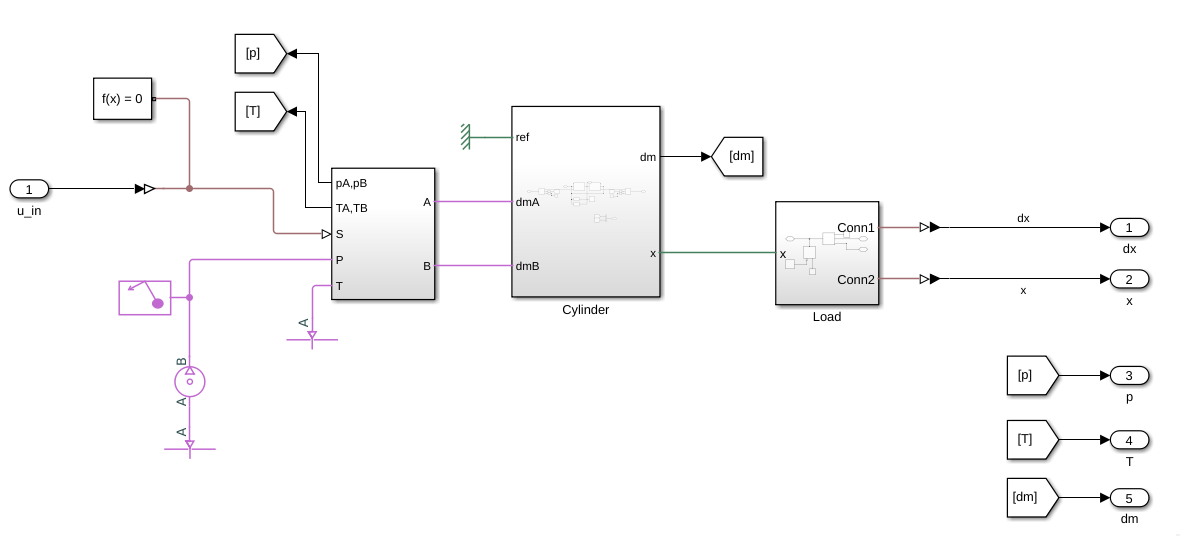
\includegraphics[width=1\textwidth]{simscape.png}
    \caption{The double-acting pneumatic piston developed using Simscape
    software}
    \label{fig:simscape}
\end{figure}


\subsection{Limitations}

It is necessary to know well the parameters of the system.

For example, we need to have a precision-measured characteristic of flow
control valve adjustment in the form of a lookup table to use a throttle
valve block.

Providing simplification and reduce the model to the only control valve,
there are still a few parameters that are not available such as valve and
dampers coefficients mentioned before \ref{}.

The main problem is the computational complexity of the model compared with
the first principle model. During the parameter estimation, the first
principle model is much faster than the Simscape model and gives an option
to experiment with different fault states analysis. 

However, both models showed quite close behavior during testing with the
same parameters; results shown in figure \ref{}.


\section{Data-Driven Models}

Between data-driven modeling techniques include:
\begin{itemize}
    \item Parametric
    \item Non-parametric
\end{itemize}

Non Parametric models include artificial neural networks and others.

% -------------------------------------------------------
%  ___ ___  _ __ ___  _ __   __ _ _ __ ___ 
% / __/ _ \| '_ ` _ \| '_ \ / _` | '__/ _ \
%| (_| (_) | | | | | | |_) | (_| | | |  __/
% \___\___/|_| |_| |_| .__/ \__,_|_|  \___|
%                    |_|                   
% -------------------------------------------------------
\chapter{Models Comparison}\label{ch:compare}

As mentioned earlier \ref{sec:digital_twin}, the simulation model can be used in several
situations.  Models of the normal condition can simulate system output to a
given input in normal operating conditions. This type of model can be used
to provide, for example, residual estimation. Compare normal condition
model with measured signals from sensors decision algorithm can evaluate
possible faults. 

Suppose the model can simulate the system in different conditions. In that
case, it gives an option to implement  "What-If" simulations and prevent
fault situations that are not captured in the measured dataset.

No best solution would apply in all situations, but for a specific example
of the double-acting pneumatic actuator with the measured dataset, the more
efficient model can be evaluated. Table \ref{tab:models_compare} represents the comparison
simulation models in 4 categories, simulation speed, accuracy concerning
the actual model, the difficulty of deploying the model, the behavior under
normal conditions and the possibility of simulating abnormal "What-If"
situations.

The speed of the simulation or calculation complexity performs a more
prominent role in the model's design, especially during the estimation of
the parameters, where the simulations are performed hundreds of times in a
row.

\begin{table}[h]
    \centering
    \begin{tabular}{|c|c|c|c|c|}
\hline
\textbf{model} &\textbf{speed} &\textbf{accuracy} &\textbf{normal cond.} &\textbf{abnormal} \\
\hline
FPM            & fast          & normal           & yes                  & yes \\
Simscape       & low           & normal           & yes                  & yes \\
HW model       & fast          & very low         & -                    & - \\
NARX           & fast          & high             & yes                  & - \\
\hline
    \end{tabular}
    \caption{Models developed by different approach comparison}
    \label{tab:models_compare}
\end{table}
    
Due to the above facts, further work was continued with the help of the
first principles model, and the development of the other models was
suspended. The first principle simulation model will be used in the next chapter
\ref{ch:mb}, PdM using Simulation Model. 
All models can be found in the attachment \textit{models}; using scripts
\textit{first\_principle\_model\_perfomance.mlx,
data\_driven\_model\_perfomance.mlx}, models can
be explored interactively.


% Artyom Voronin
%     _                     
% ___| |__  _ __  _ __ ___  
%/ __| '_ \| '_ \| '_ ` _ \ 
%\__ \ |_) | |_) | | | | | |
%|___/_.__/| .__/|_| |_| |_|
%          |_|              
%
% Brno, 2021

\documentclass[class=article, crop=false]{standalone}
\usepackage[subpreambles=true]{standalone}
\usepackage{subcaption}

\usepackage{sectsty}
\usepackage{graphicx}
\graphicspath{{img/}{../img/}{../../img/}}
\usepackage{listings}
\lstset{language=Matlab}
\usepackage{hyperref}
\usepackage{amsmath}
\usepackage{import}
\usepackage{subfiles}
\usepackage{caption}
\usepackage[utf8]{inputenc}
\usepackage[english]{babel}

%\usepackage[square, numbers]{natbib}
%\bibliographystyle{unsrtnat}
%\usepackage[nottoc]{tocbibind}

\topmargin=-0.45in
\evensidemargin=0in
\oddsidemargin=0in
\textwidth=6.5in
\textheight=9.0in
\headsep=0.25in

%\title{Preprocessing data from pneumatic actuator}
%\author{Artyom Voronin} 
%\date{}

\begin{document}
\tableofcontents

% ----------------------------------------------------------------------------- 

% ----------------------------------------------------------------------------- 

\section{Signal Based PM}
Signal-Based Predictive Maintenance.
\paragraph{General}
\paragraph{Workflow}


\subsection{Sensors}
Sensors comparison, cost.

\subsection{Data exploring}
Data has been collect from 8 types of sensors corresponding table
\ref{tab:measured_signals}:
\begin{table}[h]
    \centering
    \begin{tabular}{|c|c|}
        \hline
        Signal name                   &   Description       \\     
               \hline
           FlowExtrusin               &   Flow sensor       \\
           FlowContraction            &   Flow sensor       \\
           AirPressure                &   Pressure sensor   \\
           AccelerometerMoving\_axisY &   Accelerometer     \\
           AccelerometerMoving\_axisY &   Position encoder  \\
                                      &   Accelerometer     \\
                                      &   Temperature sensor\\
                                      &   Proximity sensor  \\
                                      &   Strain gauge      \\ 
                                      &   Microphones       \\ 
        \hline
    \end{tabular}
    \caption{Measured signals}
    \label{tab:measured_signals}
\end{table}

There are 660 measurements with different parameters system parameters
\ref{tab:params}.
\begin{table}[h]
    \centering
    \begin{tabular}{|c|c|}
        \hline
        Adjusting valve 1 &  \\
        Adjusting valve 2 &  \\
        \hline
    \end{tabular}
    \caption{Device parameters}
    \label{tab:params}
\end{table}

Dataset was divided to 5 main categories.


\begin{itemize}
\end{itemize}

Data has been accumulated to ".mat" files.
Each file contains signals from sensors during 10 seconds measurements with
different pneumatic actuator configuration. Example results from one
experiment are represented in figures \ref{fig:data_exmp1},
\ref{fig:data_exmp2}. 


\subsection{Data management}
\paragraph{Data Ensembles}
Data files have been reshaped to Data Ensembles format used for Condition
monitoring purposes. This format allows processing data without copying the
whole dataset to memory at once but processes them one by one. In large datasets
it gives an option to manipulate with data without problems with allocated memory.

\subsection{Preprocessing}
Measured signals require preprocessing concerning the preservation of the information
base. For smoothing data Moving Average function were used.
As an example, the figure \ref{fig:preprocess} is shown the "raw" and filtered signals.
The whole dataset of preprocessed data is relatively big. For
time-saving, parallel computing was used for all computationally
demanding parts of the code.


\subsection{Condition Indicators extraction}

For classification task purpose from the signals have been extracted
statistical features such as mean, median, peak to peak value, etc.
As a condition "FaultCode" variable
were used. This variable represent configuration of pneumatic actuator
during the measurement.

All calculated features were added to the dataset and were ranked by
Kruskal-Wallis ANOVA algorithm. Following table \ref{tab:feat} contain
5 first best features ranked for classification purpose.

\begin{table}[h]
    \centering
    \begin{tabular}{|c|c|c|}
        \hline
        1. & LeverPosition\_Stat\_Var & Lever position variance \\
        2. & StrainGauge\_Stat\_Mean  & Strain gauge mean value \\
        3. & StrainGauge\_Stat\_Skewness  & Strain gauge Skewness value \\
        4. & LeverPosition\_Stat\_RMS  & Lever position Root mean square
        level \\
        5. & LeverPosition\_Stat\_mean  & Lever position mean value \\ 
        \hline
    \end{tabular}
    \caption{First 5 ranked features}
    \label{tab:feat}
\end{table}

\subsubsection{Microphones}
Cheap



\subsection{Classification Task}

The main goal of the classification task is to train a model that can
predict the "FaultCode" of pneumatic actuator configuration by
calculated features.
Respecting to table \ref{feat}, the first five features have been used to
find the best classification model for our data.
Principal component analysis (PCA) has been used to reduce the number of
features and chose the best representants.
The trained model has been exported to
\textbf{models/} directory.
The confusion matrix of the trained classification model shown in figure
\ref{fig:conf}. Model accuracy on validation data is $\approx 93 \%$
\ref{fig:pred}.

\end{document}

% Artyom Voronin
%           _                     
% _ __ ___ | |__  _ __  _ __ ___  
%| '_ ` _ \| '_ \| '_ \| '_ ` _ \ 
%| | | | | | |_) | |_) | | | | | |
%|_| |_| |_|_.__/| .__/|_| |_| |_|
%                |_|              
%
% Brno, 2021

\documentclass[class=article, crop=false]{standalone}
\usepackage[subpreambles=true]{standalone}
\usepackage{subcaption}

\usepackage{xargs}
\usepackage[pdftex,dvipsnames]{xcolor}  % Coloured text etc.
\usepackage[colorinlistoftodos,prependcaption,textsize=tiny]{todonotes}

\usepackage{sectsty}
\usepackage{graphicx}
\graphicspath{{img/}{../img/}{../../img/}}
\usepackage{listings}
\lstset{language=Matlab}
\usepackage{hyperref}
\usepackage{amsmath}
\usepackage{import}
\usepackage{subfiles}
\usepackage{caption}
\usepackage[utf8]{inputenc}
\usepackage[english]{babel}

%\usepackage[square, numbers]{natbib}
%\bibliographystyle{unsrtnat}
%\usepackage[nottoc]{tocbibind}

\topmargin=-0.45in
\evensidemargin=0in
\oddsidemargin=0in
\textwidth=6.5in
\textheight=9.0in
\headsep=0.25in

%\title{Preprocessing data from pneumatic actuator}
%\author{Artyom Voronin} 
%\date{}

\begin{document}
\tableofcontents


\section{PdM using a Simulation Model (10-15 pages)}

\subsection{Differences between Model-Based PdM and PdM using Digital Twin}
There is a difference between using Model-Based PdM and using Simulation
Model as a Digital Twin.

\subsection{Model-Based Condition Indicators}
Model-Based approach is suitable when it's difficult to identify condition
indicators using only signals. In some cases it's useful to fit some model
from data and extract condition indicators as some system parameter.

\subsubsection{Static and Dynamic Models}
If the system behavior can be fit from the data as a static model, than we
can extract condition variables from this model. For example, if model
was fitting to a polynomial model, than polynomial coefficients can be use
as condition indicators.

Signals showing dynamic behavior can be fitted to dynamic models such as
State-Space or AR, ARX, NLARX (Nonlinear auto recursive model) and so on.
Then condition indicators can be extracted as poles, zeros damping
coefficients from estimated model.


\subsection{Using Simulation Model for Residuals
Estimation}\label{sec:residuals}
Another option is using the Simulink model with \textbf{prediction
error minimization function} to compute difference between Simulink model
and measured data. From this difference we can separate fault condition and
healthy operation. 


\subsubsection{Comparison with Nominal System Model}
\todo[inline]{Same thing as section \ref{sec:residuals}}

Compare actual system behavior with system model. This will generate some
error $e(t) = y(t) - \hat{y}(t)$. From this error residual can be generated
in form $r(t)=\Phi(u_t,y_t, \varepsilon_t,v_t,d)$ and after some decision.

\subsection{Using Digital Twin to Generate Fault Data}

\subsection{Using Digital Twin to Generate Prognostic Data}

\subsection{RUL}

\end{document}

\chapter{Conclusion}
The goal of this thesis was to demonstrate and verify fault detection and
predictive maintenance techniques on the double-acting pneumatic piston
assembly as a case-study object.

\section{Simulation Model}

One of the outcomes from the thesis is a simulation model of the
double-acting pneumatic piston system built based on differential equations
from the pneumatic-mechanical domain, modeled and developed using
Matlab/Simulink software. The simulation model was estimated with
parameters of healthy system behavior. However, there is an option to
reestimate parameters to fault state and simulate the system in a fault
condition. 

Due to the available measured data and significantly nonlinear dynamics of
the system, the simulation model shows good agreement with the measured
data. In contrast to the model built using Simulink/Simscape library, it is
distinctly less computationally expensive while maintaining numerical
stability. These facts are fundamental when parameter estimation is in
progress.

The simulation model was used to experiment with the system's behavior in
different conditions, model fault situations and generate data to design
and develop robust predictive maintenance algorithms. 


\section{Signal-Based PdM}
Another outcome is verifying the possibility of classification and
detection of a fault condition applying predictive maintenance techniques,
using signal-based and model-based methods.
 
The experiments were performed on a dataset measured on a demonstration
device using seven types of sensors.
  
A signal-based method is based on the extraction of useful information
directly from the signal in time-frequency domains. Each sensor required an
individual approach for preprocessing, extracting features, ranking
features and building the classification models. But generally, there is
minimal preprocessing needed to keep the possible helpful information. 

The table \ref{tab:sensors_final} contains the comparison of sensors in 2
categories, accuracy performed in the test dataset and sensor cost. The
graph \ref{fig:sensors_final_bar} visualizes these data.

Surprisingly, all sensors showed an accuracy of more than 75 \%. Microphones
offer excellent performance from a cost/accuracy perspective, and they are
suitable for installation and maintenance.

\begin{figure}[h!]
    \centering
    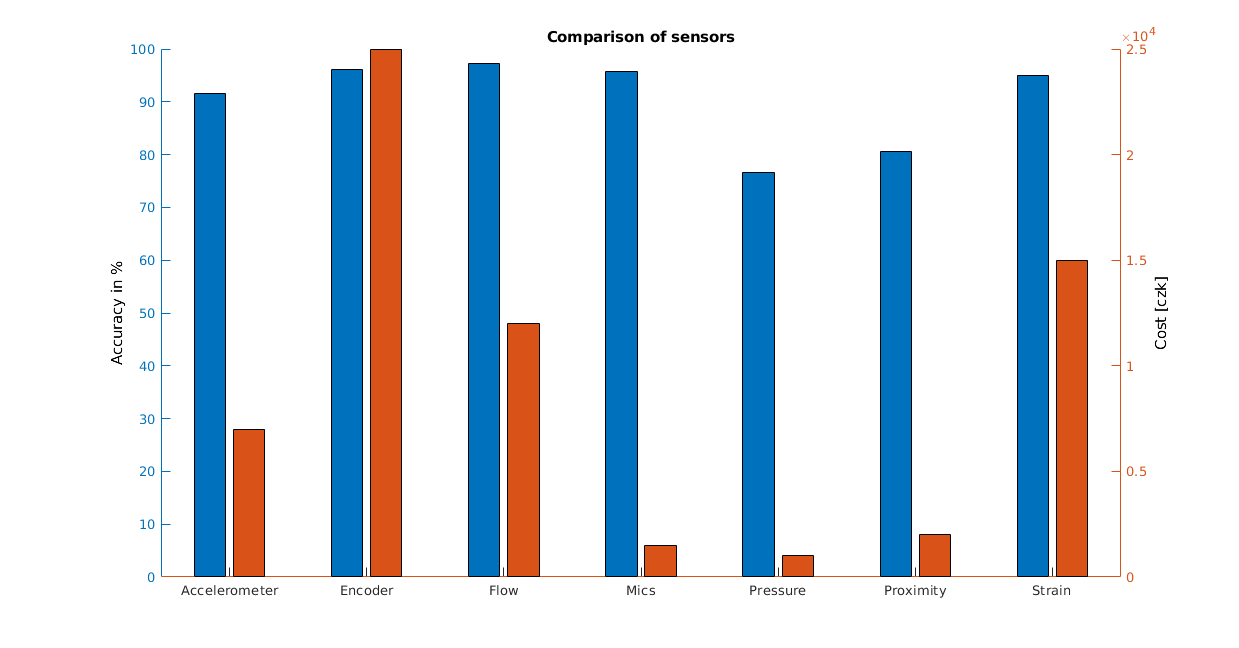
\includegraphics[width=1\textwidth]{sensors_final_bar.png}
    \caption{Comparison of sensors from accuracy/cost perspective}
    \label{fig:sensors_final_bar}
\end{figure}

\begin{table}[h]
    \centering
    \begin{tabular}{|c|c|c|c|c|c|c|c|}
        \hline
        \textbf{Sensor}   & Acc & Encoder & Flow & Mics & Pressure & Proximity & Strain \\
        \hline
        \textbf{Accuracy [\%]} & 91.6 & 96.1 & 97.2 & 95.8 & 76.6 & 80.5 & 95.0 \\
        \hline
        \textbf{Cost [czk]} & 2x 3500 & 25000 & 6000 & 3x 500 & 1000 & 2x 1000 & 15000 \\
        \hline
    \end{tabular}
    \caption{Comparison of sensors from accuracy/cost perspective}
    \label{tab:sensors_final}
\end{table}

\section{Model-Based PdM}

The next part of this thesis was to apply model-based methods and using a
simulation model for predictive maintenance algorithms. These algorithms
are practical when it is hard to extract useful information using a
signal-based method. Or it is suitable in some cases where we understand
the system dynamics and know how to exploit some system variables as
condition indicators.

The use of the method of extraction features in the form of a Nonlinear
system identification model coefficient, specifically with the
Hammerstein-Wiener model, did not give reliable results. Extracted features
have no statistical dependence, and it is impossible to predict fault type
using this method on the measured data from the pneumatic piston as a case
study.

On the other hand, the residual estimation using the simulation model
showed excellent results. The measured position signal was compared with
the signal from the simulation model in normal behavior. This residual
signal was used to classify the fault condition and achieve  99 \% on a
smaller dataset.  But given the results obtained using the signal-based
method, the residual estimation method may seem unnecessary. In this
particular case, from a practical point of view, the improvement of the
result by a few percent does not bring fundamental changes, but the
calculation time increases significantly. 

The possibility of modeling and simulation sensor faults was also verified
using the simulation model. Although it is challenging to collect fault
data from the sensor in real-life conditions, fault data can be generated
from the simulation model and even combined with the primary dataset to
create a synthetical dataset.

\subsection{RUL}
One of the main goals of predictive maintenance is to estimate the
remaining useful life. The original dataset does not contain a record of
historical data that shows degradation behavior. 

A common problem in the maintenance of pneumatic actuators is the leakage
of air from the chamber where the piston is located. This situation was
modeled on the simulation model and generated data were used for RUL
estimation. 

The generated dataset contains 25 simulations with different failure
dynamics. Each simulation includes a different number of cycles depending
on the failure dynamic before the system failure occurs.  Each cycle
contains a 10-second measurement of the system's response.  In the
experiment, a flow signal was chosen as an object of interest. From the
flow signal, the shape factor parameter was calculated and used as a
condition indicator. 

The outcome is that it is possible to estimate the remaining useful life on
generated degradation dataset by using the residual similarity model,
pairwise similarity model and linear degradation model. The prediction
results are satisfying; figure \ref{fig:rul_final} shows the linear
degradation model RUL estimation on the test data.

\begin{figure}[h!]
    \centering
    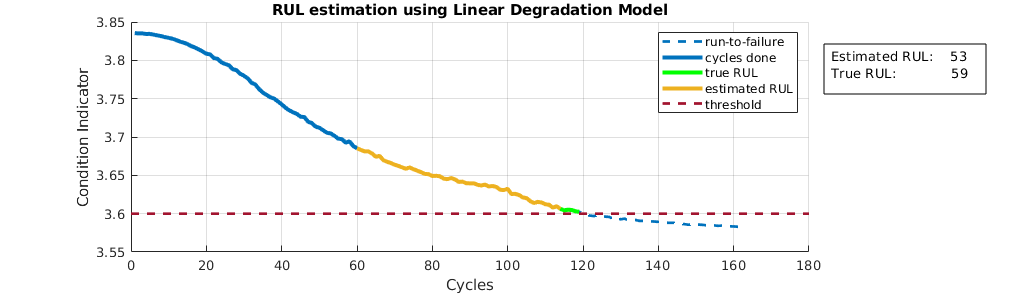
\includegraphics[width=1\textwidth]{rul_final.png}
    \caption{RUL estimation results using linear degradation model}
    \label{fig:rul_final}
\end{figure}

\section{Further Development}
As a further development, it would be appropriate to estimate the modeled
system parameters piecewise to improve the results, emphasizing the
characteristics of throttle valves and dampers with adjustments. 

Perform air leak fault condition measurements and collect historical
degradation data from a real pneumatic piston. Subsequently, evaluate the
dynamics of the failure caused by the air leak. Verify the possibility of
estimating the remaining useful life using a flow sensor. It could be an
interesting case study to verify a possibility of RUL estimation using
microphones. If the performance of the available sensors is deficient, the
pressure measurements in the chamber can be performed. The pressure in the
chamber is directly dependent on the air leakage from the chamber, as
presented in equation \ref{}. An example of pressure changes from the
simulation model is shown in figure \ref{}.


\chapter*{List of Abbreviations}
\addcontentsline{toc}{chapter}{List of Abbreviations}
\label{chap:abb}

\begin{itemize}[leftmargin=2.7cm]
	\item[\textbf{LWL}] Locally Weighted Learning
	\item[\textbf{LS}] Least Squares Method
	\item[\textbf{RLS}] Recursive Least Squares Method
	\item[\textbf{RFWR}] Receptive Field Weighted Regression
	\item[\textbf{LOLIMOT}] Local Linear Model Tree
	\item[\textbf{EGR}] Exhaust Gas Recirculation
	\item[\textbf{PID}] Proportional-Integrational-Derivative controller
	
	
\end{itemize}


\bibliography{citations.bib}
\bibliographystyle{plain}


\end{document}
